% CREATED BY DAVID FRISK, 2017

% IMPORT SETTINGS
\documentclass[12pt,a4paper,twoside,openright]{report}
% CREATED BY DAVID FRISK, 2016

\usepackage[super]{natbib}

% BASIC SETTINGS
\usepackage{moreverb}								% List settings
\usepackage{textcomp}								% Fonts, symbols etc.
\usepackage{lmodern}								% Latin modern font
\usepackage{helvet}									% Enables font switching
\usepackage[T1]{fontenc}							% Output settings
\usepackage[noconfigs, swedish]{babel}							% Language settings
\usepackage[utf8]{inputenc}							% Input settings
\usepackage{amsmath}								% Mathematical expressions (American mathematical society)
\usepackage{amssymb}								% Mathematical symbols (American mathematical society)
\usepackage{graphicx}								% Figures
\usepackage{subfig}									% Enables subfigures
\numberwithin{equation}{chapter}					% Numbering order for equations
\numberwithin{figure}{chapter}						% Numbering order for figures
\numberwithin{table}{chapter}						% Numbering order for tables
\usepackage{listings}								% Enables source code listings
\usepackage{chemfig}								% Chemical structures
\usepackage[top=3cm, bottom=3cm,
			inner=3cm, outer=3cm]{geometry}			% Page margin lengths			
\usepackage{eso-pic}								% Create cover page background
\newcommand{\backgroundpic}[3]{
	\put(#1,#2){
	\parbox[b][\paperheight]{\paperwidth}{
	\centering
	\includegraphics[width=\paperwidth,height=\paperheight,keepaspectratio]{#3}}}}
\usepackage{float} 									% Enables object position enforcement using [H]
\usepackage{parskip}								% Enables vertical spaces correctly 



% OPTIONAL SETTINGS (DELETE OR COMMENT TO SUPRESS)

% Disable automatic indentation (equal to using \noindent)
\setlength{\parindent}{0cm}                         


% Caption settings (aligned left with bold name)
\usepackage[labelfont=bf, textfont=normal,
			justification=justified,
			singlelinecheck=false]{caption} 		

		  	
% Activate clickable links in table of contents  	
\usepackage{hyperref}								
\hypersetup{colorlinks, citecolor=black,
   		 	filecolor=black, linkcolor=black,
    		urlcolor=black}


% Define the number of section levels to be included in the t.o.c. and numbered	(3 is default)	
\setcounter{tocdepth}{5}							
\setcounter{secnumdepth}{5}	


% Chapter title settings
\usepackage{titlesec}		
\titleformat{\chapter}[display]
  {\Huge\bfseries\filcenter}
  {{\fontsize{50pt}{1em}\vspace{-4.2ex}\selectfont \textnormal{\thechapter}}}{1ex}{}[]


% Header and footer settings (Select TWOSIDE or ONESIDE layout below)
\usepackage{fancyhdr}								
\pagestyle{fancy}  
\renewcommand{\chaptermark}[1]{\markboth{\thechapter.\space#1}{}} 


% Select one-sided (1) or two-sided (2) page numbering
\def\layout{2}	% Choose 1 for one-sided or 2 for two-sided layout
% Conditional expression based on the layout choice
\ifnum\layout=2	% Two-sided
    \fancyhf{}			 						
	\fancyhead[LE,RO]{\nouppercase{ \leftmark}}
	\fancyfoot[LE,RO]{\thepage}
	\fancypagestyle{plain}{			% Redefine the plain page style
	\fancyhf{}
	\renewcommand{\headrulewidth}{0pt} 		
	\fancyfoot[LE,RO]{\thepage}}	
\else			% One-sided  	
  	\fancyhf{}					
	\fancyhead[C]{\nouppercase{ \leftmark}}
	\fancyfoot[C]{\thepage}
\fi


% Enable To-do notes
\usepackage[textsize=tiny]{todonotes}   % Include the option "disable" to hide all notes
\setlength{\marginparwidth}{2.5cm} 


% Supress warning from Texmaker about headheight
\setlength{\headheight}{15pt}		





%\input{include/frontmatter/Glossaries}
\makeglossaries
 
\newglossaryentry{latex}
{
        name=latex,
        description={Is a mark up language specially suited for 
scientific documents. ORDLISTA I INNEHÅLLSFÖRTECKNING}
}

\begin{document} 

% COVER PAGE, TITLE PAGE AND IMPRINT PAGE
\pagenumbering{roman}			% Roman numbering (starting with i (one)) until first main chapter

% COVER PAGE
\begin{titlepage}
\newgeometry{top=3cm, bottom=3cm,
			left=2.25 cm, right=2.25cm}	% Temporarily change margins

% Cover page background
\AddToShipoutPicture*{\backgroundpic{-4}{56.7}{figure/auxiliary/frontpage_swe.pdf}}
\addtolength{\voffset}{2cm}

% Cover picture
\begin{figure}[H]
\centering
\vspace{0cm}	% Adjust vertical spacing here
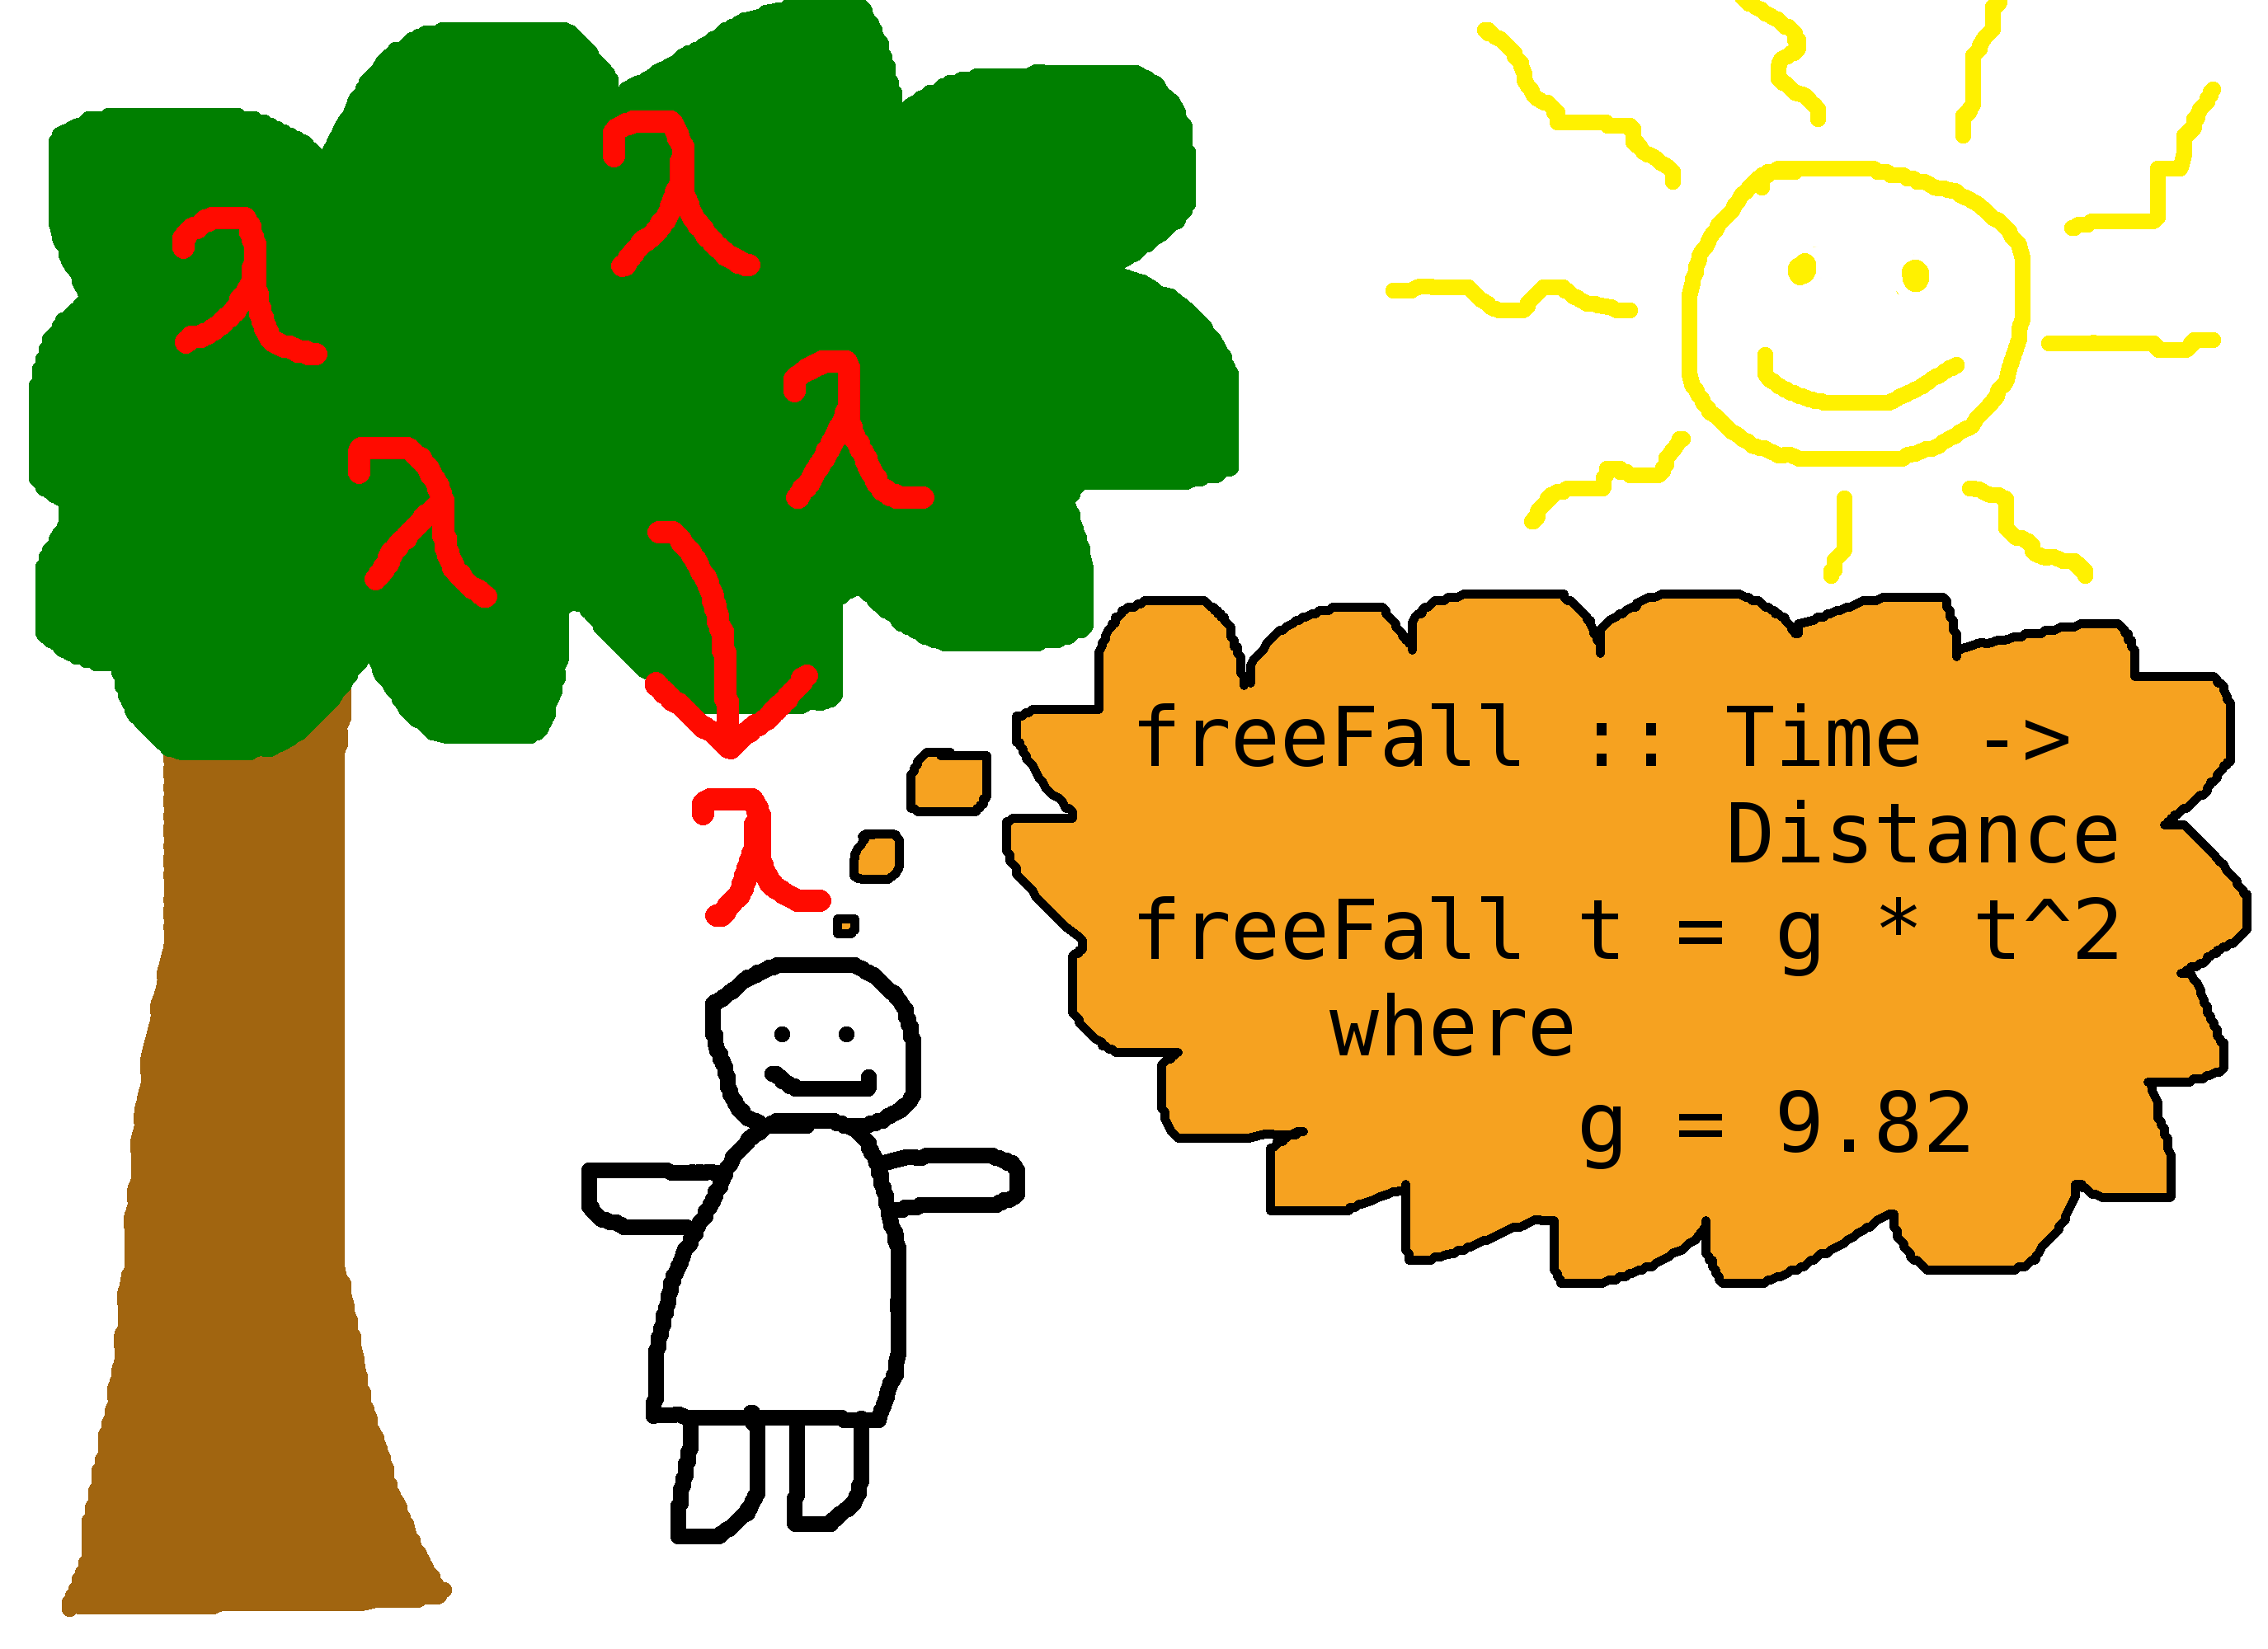
\includegraphics[width=0.99\linewidth]{figure/Framsida.png}
\end{figure}

% Cover text
%\mbox{}
%\vspace{2cm}
\renewcommand{\familydefault}{\sfdefault} \normalfont % Set cover page font
\vfill
\textbf{{\Huge  Ett alternativt läromaterial för data-\\studenter att lära sig fysik}} 	\\[0.5cm]
{\Large Läromaterialet Learn You a Physics for Great Good!}\\[0.5cm]
Kandidatarbete inom Data- och informationsteknik
\setlength{\parskip}{1cm}

{\Large Johan Johansson \\[0.3cm]
Oskar Lundström \\[0.3cm]
Erik Sjöström \\[0.2cm]
Björn Werner \\[0.2cm]}

Instutitionen för Data- och informationsteknik \\
\textsc{Chalmers tekniska högskola} \\
Göteborg, Sverige 2018

\renewcommand{\familydefault}{\rmdefault} \normalfont % Reset standard font
\end{titlepage}


% BACK OF COVER PAGE (BLANK PAGE)
\newpage
\restoregeometry
\thispagestyle{empty}
\mbox{}


% TITLE PAGE
\newpage
\thispagestyle{empty}
\begin{center}
	\textsc{\large Kandidatarbete DATX02-18-08}\\[4cm]		% Report number given by department
	\textbf{\Large Ett alternativt läromaterial för datastudenter att lära sig fysik} \\[1cm]
	{\large Läromaterialet Learn You a Physics for Great Good!}\\[1cm]
	{\large Johan Johansson}\\
  {\large Oskar Lundström}\\
 	{\large Erik Sjöström}\\
  {\large Björn Werner}\\

	\vfill
	% Logotype on titlepage
	\begin{figure}[H]
	\centering
	% Remove the following line to remove the titlepage logotype
	
\includegraphics[width=0.2\pdfpagewidth]{figure/auxiliary/logo_swe.pdf} \\
	\end{figure}	\vspace{5mm}

	Instutionen för Data- och informationsteknik \\
	\emph{Avdelningen för funktionell programmering}\\
	\textsc{Chalmers tekniska högskola} \\
	Göteborg, Sverige 2018 \\
\end{center}


% IMPRINT PAGE (BACK OF TITLE PAGE)
\newpage
\thispagestyle{plain}
\vspace*{0cm}
Ett alternativt läromaterial för datastudenter att lära sig fysik\\
Läromaterialet Learn You a Physics for Great Good!\\
Johan Johansson \\
Oskar Lundström \\
Erik Sjöström \\
Björn Werner
\setlength{\parskip}{1cm}

\copyright ~ Johan Johansson, 2018. \setlength{\parskip}{1cm} \\
\copyright ~ Oskar Lundström, 2018. \setlength{\parskip}{1cm} \\
\copyright ~ Erik Sjöström, 2018. \setlength{\parskip}{1cm} \\
\copyright ~ Björn Werner, 2018. \setlength{\parskip}{1cm}

Handledare: Patrik Jansson, CSE, Chalmers\\
Examinator: Nils Anders Danielsson, CSE, Chalmers \setlength{\parskip}{1cm}

Kandidatarbete DATX02-18-08 \\
Instutionen för Data- och informationsteknik \\
Avdelningen för funktionell programmering\\
Chalmers tekniska högskola\\
SE-412 96 Göteborg\\
Telefon +46 31 772 1000
\setlength{\parskip}{0.5cm}%TODO: why set it here?

\vfill
% Caption for cover page figure if used, possibly with reference to further information in the report
Omslag: Newton står och tänker på fritt fall i termer av Haskellkod och precis då får han ett lambda-äpple i huvudet. Bilden är ritad i samma stil som bilderna i läromaterialet.

Typsatt i \LaTeX \\
Göteborg, Sverige 2018


% ABSTRACT
\newpage
%TODO: Make sure to define a macro for the headline once and for all. Then reuse it when needed.
\setlength{\parskip}{0.5cm}

\thispagestyle{plain}			% Supress header
\section*{Abstract}

% max 150 ord typ
\begin{binge}

%https://www.sfu.ca/~jcnesbit/HowToWriteAbstract.htm
% Punktlista på vad som ska vara med:
% 150 ord max
% whole thesis -> condenced form

% Snott från sammandrag:




% Building blocks:    
%   En mening om varje kapitel:
    Introduction (sv introduktion): Describes the starting point, goals and restrictions.
    Theory (sv. teori): Describes concepts of DSL, functional programming and learning models aimed for the learning material.
    Method (sv. genomförande): Describes the construction of the material, publishing, the procedure of testing with a testgroup and comments from keyfigures from the ordinary education.
    Results (sv. resultat): Describes the resulting material, the feedback from the testgroup and the comments from a physic teacher.
    Discussion (sv. diskussion): Reviews the methodology and the results. Also mentions possible further extensions and ethical dimensions of the material.
    Conclusions (sv. slutsatser): A final summary connecting the initial goals, with the methodology, and the result.


% KEYWORDS (MAXIMUM 10 WORDS)
\vfill
Keywords: Läromaterial, fysik, haskell, funktionell programmering.
\end{binge}
% Learning material, physics, haskell, functional programming.

\newpage				% Create empty back of side
\thispagestyle{empty}
\mbox{}


% SAMMANFATTNING
\newpage

\thispagestyle{plain}			% Supress header

%TODO: Perhaps include both Abstract + Sammanfattning on one page?

\section*{Sammanfattning}
TODO: Lorem ipsum dolor sit amet, consectetur adipisicing elit, sed do eiusmod tempor incididunt ut labore et dolore magna aliqua. Ut enim ad minim veniam, quis nostrud exercitation ullamco laboris nisi ut aliquip ex ea commodo consequat. Duis aute irure dolor in reprehenderit in voluptate velit esse cillum dolore eu fugiat nulla pariatur. Excepteur sint occaecat cupidatat non proident, sunt in culpa qui officia deserunt mollit anim id est laborum.

% KEYWORDS (MAXIMUM 10 WORDS)
\vfill
TODO: Keywords: lorem, ipsum, dolor, sit, amet, consectetur, adipisicing, elit, sed, do.

\newpage				% Create empty back of side
\thispagestyle{empty}
\mbox{}

% ACKNOWLEDGEMENTS
\newpage
\thispagestyle{plain}			% Supress header
\section*{Förord}

\begin{draft}

Denna rapport behandlar kandidatarbetet ``Matematikens domänspecifika språk'',
som genomfördes på Chalmers tekniska högskola under vårterminen 2018. Vi som har
utfört detta kandidatarbete är tre studenter från civilingengörsprogrammet
Datateknik vid Chalmers tekniska högskola och en student från det
datavetenskapliga programmet vid Göteborgs Universitet.

Vi vill tacka Patrik Jansson, vår handledare, som med sina kloka tankar och goda
råd agerat som ett fyrtorn när vi seglat på okända domänspecifika hav. Vi vill
tacka Åke Fäldt som tagit sig tiden att diskutera sin egen kurs, vårt
läromaterial och gett oss tips och råd under utvecklingen. Vi vill tacka de
testare, både individer och grupper, som tagit sig tiden att studera och läsa
igenom vårt, ibland halvfärdiga, material och gett oss den kritik vi behövde för
att sporras till vidareutveckling. Vi vill tacka Jeff Chen vars tankar och idéer
om potentiella vidareutvecklingar för projektet gav oss ett helt nytt perspektiv
under arbetets gång.

Slutgiltligen vill vi tacka Miran Lipovača vars hemsida ``Learn You a
Haskell for Great Good!'' har både inspirerat utformningen av vår hemsida och
agerat som ett läromaterial för våra egna inledande studier av det fantastiska
programmeringsspråket Haskell. 

\end{draft}

\vspace{1.5cm}
\hfill
Författarna, Göteborg, Maj 2018.

\newpage				% Create empty back of side
\thispagestyle{empty}
\mbox{}



% TABLE OF CONTENTS
\newpage
\tableofcontents

% OTHER FRONTMATTER
% List of figures (add to table of contents)
\cleardoublepage
\addcontentsline{toc}{chapter}{\listfigurename} 
\listoffigures
% List of tables (add to table of contents)
\cleardoublepage
\addcontentsline{toc}{chapter}{\listtablename}  
\listoftables
% Ordlista
\cleardoublepage
% \addcontentsline{toc}{chapter}{Ordlista}
% 
\chapter*{Ordlista}
\markboth{Ordlista}{}

\todo{I bokstavsordning när vi har med alla ord vi ska.}

\textbf{DSL} Förkortning av \textit{Domain Specific Language}, engelska för domänspecifikt språk.

\textbf{Grundläggande område} Ett område i läromaterialet som inte bygger på något annat område. Till exempel vektorer.

\textbf{Komposit område} Ett område i läromaterialet som bygger på andra områden. Till exempel lutande plan, som använder sig av vektorer.

\textbf{Åke Fäldt} Föreläsare och examinator i kursen Fysik för ingenjörer.

\textbf{Fysik för ingenjörer} En fysikkurs som är obligatorisk för studenter på Datateknik civilingenjör på Chalmers. Den ges i årskurs 2 och innehåller grunderna i klassisk mekanik, termodynamik och vågrörelselära.

\textbf{Univerisity Physics} Den fysikbok som används i Fysik för ingenjörer.

\textbf{Läromaterialet} Syftar på den pedagogiska text som projektet resulterat i.

\textbf{Litterate Haskell} Litterat programmering i Haskell. Se avsnitt \ref{sec:lhs}

\textbf{Syntax} Grammatiken för ett språk, som beskriver hur man konstruerar meningar i det. Se avsnitt \ref{sec:syntax}.

\textbf{Semantik} Vad meningar (skapade i en syntax) har för betydelse. Se avsnitt \ref{sec:syntax}.

\textbf{Syntaxträd} En trädrepresentation av syntax. Se avsnitt \ref{sec:syntax}

\textbf{Fysikläraren} Åke Fäldt.
  

\printglossary[type=\acronymtype]
 
\printglossary


% START OF MAIN DOCUMENT
\cleardoublepage
\setcounter{page}{1}
\pagenumbering{arabic}			% Arabic numbering starting from 1 (one)
\setlength{\parskip}{\baselineskip}


\chapter{Introduktion}

Detta kapitel beskriver projektets bakgrund, mål och avgränsningar.

\section{Bakgrund}

På civilingenjörsprogrammet Datateknik på Chalmers tekniska högskola ingår den
obligatoriska fysikkursen \textit{Fysik för ingenjörer}. Tentastatistiken för
denna kurs~\cite{tentastatistik} är ganska dålig\footnote{Andel underkända på ordinarie tentamen från läsår 2014 till
2017: 34\%, 76\%, 18\%, 57\%.}. Vi tror att många studenter på
Datateknik tycker att denna kurs är svår eller ointressant och att detta leder
till att en betydande andel får underkänt.

Detta tror vi kan lösas med avstamp från kursen \textit{Domain
Specific Languages of Mathematics} (``DSLsofMath''), med den svenska titeln
\textit{Matematikens domänspecifika språk}. Kursen är valbar på kandidatnivå för studenter på Chalmers och Göteborgs universitet. Konkret
presenterar DSLsofMath matematik som derivator, komplexa tal och
matriser ur ett programmeringsperspektiv i Haskell, vilket är ett programmeringsspråk datastudenterna redan är bekanta med.

DSLsofMath-kursens skapare, Cezar Ionescu och Patrik Jansson, har beskrivit avsikten med kursen i en artikel~\cite{tfpie2015}. Det direkta målet med kursen är
att förbättra den matematiska utbildningen för datavetare och den
datavetenskapliga utbildningen för matematiker, där den grundläggande idén
bakom kursen är:

\begin{center} ``[\dots] att uppmuntra studenterna att närma sig matematiska
  domäner från ett funktionellt programmeringsperspektiv: att ge beräkningsbevis
  (calculational proofs); att vara uppmärksamma på syntaxen för matematiska
  uttryck; och, slutligen, att organisera de resulterande funktionerna och
typerna i domänspecifika språk.''~\cite{tfpie2015}
\end{center}

Det programmeringsperspektiv som kursen använder sig av bottnar i
så kallade domänspecifika språk. Kortfattat kan ett domänspecifikt språk
beskrivas som ett programmeringsspråk som skapats för ett väl avgränsat
område. Detta område kan vara databashantering, algebraiska uttryck eller till
och med fysik. Språket kan antingen vara implementerat inuti ett annat
programmeringsspråk eller implementerat helt fristående. I kursen och projektet
är de implementerade i Haskell.

Idén bakom projektet är att använda domänspecifika språk för att ur ett alternativt perspektiv presentera fysik. Likt det sätt DSLsofMath
presenterar kopplingar mellan matematik och programmering ska projektet på motsvarande sätt visa på kopplingar mellan programmering och fysik och därmed
underlätta lärandet. För att förtydliga ges här en analogi:

%PaJa:Trevligt!

\begin{center}
Studenterna har svårt för matematik $\rightarrow $ DSLsofMath.\\
Studenterna har svårt för fysik $\rightarrow $ Detta projekt.
\end{center}

Detta projekt kan vara av intresse för studenter, pedagoger och
föreläsare inom de berörda områdena eftersom projektet ger ett nytt
perspektiv på fysik som inte bara är annorlunda utan också mer rigoröst.
Förhoppningsvis blir det även relevant för de som är intresserade av
domänspecifika språk i stort och kanske till och med för programledningen som
kan se denna rapport som ett skäl att introducera innehåll av detta slag i
fysikkurser.

Angående tidigare forskning och studier har en kurs på MIT, inte helt olik
DSLsofMath, tidigare givits som berör både fysik och
domänspecifika språk.
%funktionell programmering.
\textit{Classical Mechanics: A Computational Approach} gavs av Gerald Sussman
och Jack Wisdom senast år 2008~\cite{classical-mechanics-course-mit-2008}.
Denna kurs på avancerad nivå behandlar de fundamentala principerna för klassisk
mekanik med hjälp av beräkningsidéer för att precist formulera principerna av
mekanik, med början i Lagranges ekvationer och avslut i perturbationsteori
(teori för approximationer av matematiska lösningar). I kursens bok~\cite{SICM}
förklaras fysikaliska fenomen genom att visa datorprogram för att simulera dem,
skrivna i språket Scheme. Denna typ av kurs är ovanlig och är, till
projektgruppens kännedom, den enda kursen bortsett från DSLsofMath som knyter
samman fysik, programmering och matematik på en symbolisk nivå för att förklara
koncepten.

Även tidigare har det genomförts ett kandidatarbete på Chalmers med anknytning till DSLsofMath.
Vårterminen 2016 genomfördes kandidatarbetet \textit{Programmering som
undervisningsverktyg för Transformer, signaler och system. Utvecklingen av
läromaterialet TSS med DSL} av fem studenter från Datateknik och Teknisk
Matematik på Chalmers~\cite{kandidat2016}. Arbetet bestod av utveckling av läromaterial med
tillhörande programmeringskod, uppgifter och lösningar, som komplement till
existerande kurser i signallära.

Till sist finns det ett arbete som liknar detta arbete i både syfte och
programmeringsspråk, vilket utfördes av Scott N. Walck vid Lebanon Valley
College~\cite{lebanon-physics}. Syftet med det projektet var att fördjupa
studenters förståelse av fysik, med fokus på elektromagnetisk teori, genom att
uttrycka fysiken med hjälp av funktionell programmering.

\section{Projektets mål}

Målet med detta kandidatarbete är att angripa fysik från ett
programmeringsperspektiv, förhoppningen är då att fysik ska bli både
roligare och intressantare för datastudenter, och därmed också
enklare. Detta liknar premissen bakom kursen DSLsofMath och kandidatarbetet
från 2016, som istället för fysik behandlade matematik respektive signallära.

Mer konkret ska målet ovanstående uppnås genom att skapa ett läromaterial.
Läromaterialet ska bestå av
domänspecifika språk som modellerar fysik, skrivna
%programkod skriven
i Haskell,
sammanvävt med en förklarande lärotext. Läromaterialet ska vara
enkelt för läsaren att ta till sig, vilket ska åstadkommas genom ett lättsamt
språk, publicering på en hemsida samt fri tillgång till källkoden.

Ett parallellt mål är att, efter att ha tillägnat sig erfarenhet, diskutera
huruvida fysik och domänspecifika språk går att kombinera och om det finns en
pedagogisk nytta i att göra det.

\section{Avgränsningar}\label{sec:avgransningar}

Läromaterialet begränsas till att enbart hantera de fysikaliska områden
som ingår i kursen Fysik för ingenjörer. Denna avgränsning valdes dels eftersom
det är den fysik gruppmedlemmarnas kunskaper är begränsad till, och dels för att
det är denna kurs som projektet kan bli mest relevant för, eftersom
kursen ingår i datastudenternas obligatoriska kursplan.

Vidare ska en prioritering av innehållet i Fysik för ingenjörer göras.
Kursen behandlar grunderna inom klassisk mekanik, termodynamik och
vågrörelselära samt en stor mängd tillämpad matematik, exempelvis
differentialkalkyl. I första hand behandlas mekaniken, för att sedan i mån
av tid även behandla termodynamik och vågrörelselära. Fokuset läggs även
på de områden datastudenter haft svårt för.

För att pröva den pedagogiska nyttan kommer enbart en informell testning
att göras. Detta då en rigorös undersökning hade krävt mycket tid för att välja
lämpliga testgrupper, analysera återkopplingen samt dokumentera
testningsförloppet. Denna tid läggs istället på att skapa ett intressant innehåll.

Projektet fokuserar mer på att skapa innehåll än att göra
efterforskningar på, och tillämpa, pedagogiska teorier och riktlinjer. Denna
avgränsning valdes eftersom det är hur innehållet kan se ut som är
intressant och nytt, inte hur ett pedagogiskt läromaterial kan skrivas på bästa sätt. Den
pedagogiska aspekten kommer inte ignoreras helt, fokuset på den kommer bara att
vara mindre.



\chapter{Teori}

I detta kapitel beskrivs fyra koncept av central betydelse för projektet. Dessa
koncept är domänspecifika språk, begreppen syntax, syntaxträd och semantik,
litterat programmering samt lärandeteorier.

\section{Domänspecifika språk}

Ett domänspecifikt språk är ett språk som är avgränsat till en specifik domän.
Nyckelorden är språk, specifik och domän. En domän är ett område, till exempel
textformatering eller matlagning. Specifikt syftar det på att det är \textit{just
detta} område man lägger fokus på. Med språk menas ett sätt att uttrycka
saker inom domänen. Svenska och Java är två exempel på språk.

Domänspecifika språk är vanligt förekommande i programmeringssammanhang. HTML är
ett domänspecifikt språk för textformatering, SQL för databashantering och
CSV för tabeller. Precis som domänspecifika språk i vardagen passar
domänspecifika språk inom programmering bäst för sin egen domän. SQL är bra för
att hantera en databas men inte för att skapa ett spel.

Domänspecifika språk används inte bara i programmering utan förekommer även i
andra mer vardagliga sammanhang. Inom domänen matlagning är steka, grilla och
fritera användbara ord. Likaså inom domänen ridning är grimma, box och galopp
användbara ord. Befinner man sig inom domänen vet man vad som menas med grimma
och det är ett kort och väldefinierat sätt att uttrycka sig. Men detta språk (här
i form av ord och begrepp) blir svårtolkat utanför domänen. Ett recept kan inte
förklaras i termer av grimmor, boxar och galopper.

Motsatsen till ett domänspecifikt språk är ett generellt språk. I
vardagen är naturliga språk som svenska och engelska generella medan
ryttar-begreppen ovan är domänspecifika. Precis som i vardagen finns
det i datavärlden generella programmeringsspråk, till exempel C++ och
Java. Dessa är turingkompletta, vilket betyder att det går att
uttrycka alla beräkningsbara problem i dem och även lösa dem givet
tillräckligt med tid och
minnestillgångar~\cite{turing_ne}~\cite{turing_book}. Nackdelen med
dessa generella språk är just att de är så generella. Eftersom
domänspecifika språk inte behöver vara användbära utanför den
specifika domänen kan de inkludera speciell syntax och ha inbyggd
funktionalitet som inte hade passat i ett generellt språk.

Ett domänspecifikt språk kan antingen implementeras som ett fristående språk
eller bäddas in i ett redan existerande språk. De domänspecifika språk som
utvecklats inom detta projekt är inbäddade i programmeringsspråket
\textit{Haskell}. Haskell är ett lämpligt val eftersom det är enkelt att skapa
datatyper som bygger upp det domänspecifika språket. Att Haskell är ett
högnivå-språk är också en fördel då man slipper programmeringstekniska detaljer,
till exempel minneshantering, och istället kan fokusera på programmets innehåll
och betydelse. Slutligen gör dess mönstermatchning att de datatyper som utgör
det domänspecifika språket enkelt kan brytas isär och manipuleras.

För vidare läsning om domänspecifika språk rekommenderas \textit{DSL for the Uninitiated} \cite{DSLU}. 

\section{Syntax, syntaxträd och semantik}\label{sec:syntax}

I samband med domänspecifika språk dyker begreppen \textit{syntax} och
\textit{semantik} upp. Syntax är reglerna för hur man sammanslår
enheter, som ord, i språket till komplexa strukturer, som meningar och
satser. Semantik är betydelsen av sådana komplexa strukturer i ett språk.
Inom aritmetik\footnote{Aritmetik är
  den gren inom matematiken som behandlar räkning av tal.} är tal och
operationer syntax medan värdet av uttrycket är semantiken.  Till
exempel har det syntaktiska uttrycket $((3 + 2) * 10)^4$ det semantiska värdet $6.250.000$,
eftersom det är det som det syntaktiska uttrycket \textit{betyder}.
Domänspecifika språk har med syntax att göra eftersom många
domänspecifika språk används för att modellera just syntax.

I domänspecifika språk som modellerar syntax, så kallade \textit{deep
embeddings}, kan syntaxen representeras av trädstrukturer. Dessa
strukturer kallas *syntaxträd*, och har haft stor betydelse i detta projekt.
För att illustrera begreppet visas här ett domänspecifikt språk som består av ett
syntaxträd som modellerar aritmetiska uttryck, implementerat i Haskell.
Datatypen för syntaxträdet visas i figur~\ref{fig:syntax_exempel}.

\begin{figure}[tph]
  \begin{lstlisting}
data Expr = Expr :+: Expr
          | Expr :*: Expr
          | Const Double
  \end{lstlisting}
  \caption{En datatyp för aritmetiska uttryck i Haskell. Detta är ett exempel på
           ett litet domänspecifikt språk.}\label{fig:syntax_exempel} 
\end{figure}

Typen innehåller \textit{datakonstruktorer} för att representera
\textit{löv} (ändpunkter) och \textit{förgreningar}. I detta exempel är
\texttt{:+:} och \texttt{:*:} förgreningar. Med hjälp av dem kan man uttrycka
summan respektive produkten av två andra uttryck. Löven representeras av
\texttt{Const}. Det är en konstant som man ej kan bygga vidare på.

Med datakonstruktorerna kan man konstruera uttryck representerade av syntaxträd. Ett exempeluttryck
från den tidigare datatypen visas i figur~\ref{fig:syntax_exempel_varde}, som visar hur det aritmetiska uttrycket $7 * (3
+ 10)$ modelleras. Konstruktorn \texttt{:*:} får som sina två argument uttrycken
\texttt{Const 7} och \texttt{Const 3 :+: Const 10}. Det är alltså en produkt av
två deluttryck. Syntaxträd brukar illusteras med träddiagram. Detta
exempeluttryck illustreras i figur \ref{fig:syntax_exempel_bild}.

\begin{figure}[tph]
  \begin{lstlisting}
expr = Const 7 :*: (Const 3 :+: Const 10)
  \end{lstlisting}
  \caption{Ett exempeluttryck ur det tidigare syntaxträdet. Detta modellerar det
           matematiska uttrycket $7 * (3 + 10)$}\label{fig:syntax_exempel_varde}
\end{figure}

\begin{figure}[tph]
  \centering
  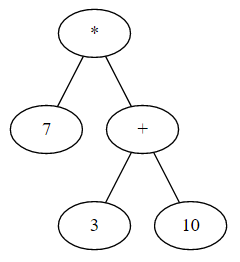
\includegraphics[width=0.4\linewidth]{figure/syntax_exempel_bild.png}
  \caption{Ett exempeluttryck från syntaxträdet illustrerat i ett
           träddiagram.}\label{fig:syntax_exempel_bild} 
\end{figure}

Precis som semantik har en roll i samband med syntax, har semantik även en roll
i samband med syntaxträd. I detta exempel är semantiken det värde som
syntaxträdet har. Detta värde kan beräknas utifrån syntaxträdet genom
en \textit{evaluator}, också kallad \textit{beräkningsfunktion}. För exemplets
syntaxträd kan beräkningsfunktionen se ut som i figur \ref{fig:eval_tree}

\begin{figure}[tph]
  \begin{lstlisting}
evaluate :: Expr -> Double
evaluate (e1 :+: e2) = evaluate e1 + evaluate e2
evaluate (e1 :*: e2) = evaluate e1 * evaluate e2
evaluate (Const v)   = v
  \end{lstlisting}
  \caption{En beräkningsfunktion för syntaxträdet.}\label{fig:eval_tree}
\end{figure}

Det finns tre speciella saker att observera i
figur~\ref{fig:eval_tree}. Den första är att eftersom syntaxen innehåller tre olika
slag av element, här motsvarat av de tre datakonstruktorerna, krävs tre fall i
beräkningsfunktionen som beräknar vardera av dem. \texttt{evaluate} har
därför ett fall för \texttt{:+:}, ett för \texttt{:*:} och ett för
\texttt{Const}. 

Den andra saken att notera i figuren är hur ett fall
beräknas. Hur beräkningen ska se ut får man genom att ta hänsyn till
semantiken hos det syntaktiska uttrycket. \texttt{e1 :+: e2} är syntax för
addition av de två uttrycken \texttt{e1} och \texttt{e2}. Därför blir
semantiken, värdet, av \texttt{e1 :+: e2} lika med värdet hos \texttt{e1} och
\texttt{e2} adderade. Ett liknande resonemang ger svaret på hur beräkningen av
de två resterande fallen ska se ut.

Den tredje saken värd att poängtera är beräkningsfunktionens
typsignatur, \texttt{Expr -> Double}. Den gör nämligen att man kan tolka
\texttt{evaluate}, och beräkningsfunktioner i allmänhet, som en översättning
från syntax (här \texttt{Expr}) till semantik (här \texttt{Double}).

\section{Litterat programmering och Literate Haskell}\label{sec:lhs}

\textit{Litterat programmering} (engelska \textit{literate programming}) är ett
alternativt sätt att programmera som introducerades av Donald Knuth~\cite{knuth}.
Istället för att skriva ett program främst för datorer att exekvera, så skriver man
programmet främst för människor att läsa.

Jämfört med traditionella program får dokumentationen en
ökad betydelse. I traditionella program är programkoden den viktiga delen. I
litterata program är däremot dokumentationen minst lika viktig. Den används till
att förklara koden, sätta den i relationen till andra delar, med mera.
Detta jämnbördiga förhållande syns konkret genom att titta på hur källkoden är
skriven i ett litterat program. Det kan till exempel se ut som i
figur~\ref{fig:litterate_haskell_exempel} där man ser att källkoden och
dokumentationen är sammanvävda på ett jämnbördigt sätt, där den ena inte är
viktigare än den andra.

\begin{figure}[tph]
  \begin{lstlisting}[language={}]
How does all this tie together? First the type is decided, for instance

> type ExampleType = Quantity T.Length Double

then a value of that type is created

> exampleValue :: ExampleType
> exampleValue = Quantity V.length 5.3

Note that the Quantity data type has both value-level and type-level dimensions. As previosuly mentioned, value-level in order to pretty print and type-level to only permit legal operations.
\end{lstlisting}
  \caption{Ett exempel på hur en källfil till litterat programmering kan se ut, tagen direkt från källkoden till läromaterialet.
           I exemplet är koden skriven i Literate Haskell. Rader som börjar med \texttt{>}
           markerar att det är programkod, medan rader utan markerar att det är
           dokumentation.}\label{fig:litterate_haskell_exempel} 
\end{figure}
% OBS! Raden med "note that the quantity..." måste vara en lång rad. Annars blir det fel i PDF:en

%Det andra sättet ett litterat program skiljer sig åt är ordningen programkoden
%står i. Traditionell programmering börjar oftast med att definiera små funktioner
%och metoder med snäva användningsområden och använder sedan dessa för att senare
%bygga ihop mer komplexa strukturer. Med litterat programmering börjar man hellre
%med komplexa strukturer först och skriver text som förklarar den generella
%strukturen utan att gå in på detaljerna, för att sedan presentera de små
%delarna var för sig med tillhörande förklarande text.

\textit{Literate Haskell} är litterat programmering för Haskell~\cite{litterate_haskell}.
Att programmera i Literate Haskell går till på samma sätt som vanlig Haskell,
med skillnaden att programkod och text vävs ihop i en och samma fil. Det kan
se ut som i figur~\ref{fig:litterate_haskell_exempel}. Filen, med tillägget
\texttt{.lhs}, går att använda direkt med Haskell-kompilatorn GHC. All text
ignoreras och programkoden behandlas som om den var en vanlig
Haskell-fil. Filen kan också kompileras till en läsbar typsatt rapport eller hemsida.
Det finns flera verktyg som gör det men det som används i detta
projekt är \textit{Pandoc}~\cite{pandoc}. Med Pandoc kan texten märkas
upp med både \textit{Markdown} (används i projektet) och \LaTeX. Det går
att exportera till bland annat HTML (som i läromaterialet) och PDF (som i den här rapporten).


\section{Att skapa motiverande läromaterial}\label{sec:arcs}

Motivation är en persons vilja att göra något och i undervisningssammanhang vill
man att studenten ska lära sig materialet. Studenten behöver alltså vara
motiverad, ha vilja att, lära sig. Motivation kan ha flera källor, till exempel att
studenten tycker materialet är intressant eller att det finns belöningar i form
av tillfredsställelsen att få att högt betyg. 

\textit{Motiverande design} innebär att systematiskt utforma undervisningen på
ett sådant sätt att studenten blir motiverad till att lära sig. Det handlar om
att använda olika tekniker för att väcka och behålla motivation. Det finns ett
flertal olika modeller för detta men i detta projekt används enbart den så
kallade \textit{ARCS-modellen}~\cite{arcs_book}.

\textit{ARCS} är en förkortning av ``Attention, Relevance, Confidence and
Satisfaction'', på svenska ``uppmärksamhet, relevans, självförtroende och
tillfredsställelse''. Precis som namnet antyder innehåller modellen fyra delar
som vardera behandlar en aspekt av motivation. \textit{Attention} handlar om att
fånga uppmärksamhet och väcka nyfikenhet. \textit{Relevance} handlar om att
tillgodose studentens behov så att materialet upplevs som relevant.
\textit{Confidence} handlar om att övertyga studenten att hen kan
lyckas lära sig materialet. \textit{Satisfaction} handlar om att ge studenten
tillfredsställelse efter att ha lärt sig något så att hen vill fortsätta lära
sig. Det finns olika strategier för hur man genomför de olika delarna i praktiken och
här följer en översikt för \textit{Attention}.\footnote{Eftersom projektet har
ett begränsat fokus på de pedagogiska aspekterna, se
avsnitt~\ref{sec:avgransningar}, har enbart \textit{Attention}  tagits hänsyn till. Av detta skäl är det enbart denna
del beskriven här.}

För att fånga studentens uppmärksamhet och intresse finns tre allmänna
strategier. Den första är varseblivning, att något plötsligt händer som man
blir medveten om. Det kan till exempel åstadkommas genom överraskande
information, en förändring i ljuset i en föreläsning eller att humor vävs in.
Den andra är att väcka nyfikenhet. Ett par sätt för det är att involvera mystik
i miljön och att ställa frågor. Det tredje sättet är variation. Då handlar det
om olika struktur och ordning på utlärningen, till exempel att inte alltid
utforma en lektion som föreläsning, demonstration och sedan övning, utan variera
det med andra inslag, exempelvis ett filmklipp.

Utifrån det sociokulturella perspektivet som Vygotskij utvecklade~\cite{LSB_und}
lär sig elever av varandra. Eleverna befinner sig vid sin närmsta 
utvecklingszon, där eleverna kan hjälpa varandra att förstå innebörden av
definitioner och uttryck genom att sätta ord på det de vill kommunicera. Denna
typ av kommunikation kan hjälpa elever sätta fingret på vad de
inte förstår. Med denna bakgrund kan parprogrammering vara
fördelaktigt. Dels för att eleverna kan lära sig av varandra, att de genom att
kommunicera sin förståelse internaliserar ämnet och bygger en djupare
förståelse. Parprogrammering kan även lämpa sig för att begränsa
flyktförsök, där elever medvetet eller mindre medvetet börjar göra något annat.

%Jean Piaget - Kognitivismen (lära sig A, B, A + B -> C, alternativt att eleven utmanas med något den trodde var sant, och tvingas omformulera en lösning som stödjer den presenterade situationen). s157

Två andra aspekter på lärande är interaktion och snabba
belöningar. Eftersom internetplattformars interaktion med eleven är
begränsad i jämförelse med då eleven är i skolan och har tillgång till
lärare, så brukar internetbaserade läroplattformar förlita sig på
behavioristiska element (former av respons) i form av rätt eller fel
svar~\cite{LSB_und}. Evolutionärt sett har snabba belöningar varit
fördelaktigt framför långsiktiga som kräver långsiktigt engagemang
(exempelvis öva inför en tenta) vilket beskrivs i boken \textit{Dansa
  på deadline: Uppskjutandets psykologi}~\cite{DPD}.


% Metoddelen redogör för vad du gjort och hur du gått tillväga; det är
% en beskrivning av den metod som ligger till grund för det du kommit
% fram till och hävdar i din rapport.

% Beskrivningen i metoddelen ska vara koncis snarare än helt
% uttömmande men ska samtidigt göra det möjligt att upprepa studien

% Metoddelen ska inte vara en omgjord labbinstruktion och den ska inte
% heller innehålla teori med mindre än att teoretiska hänsyn har haft
% en direkt inverkan på metoden.

% Metoddelen skrivs nästan alltid i dåtid (imperfekt) och ofta används
% passiv form för att beskriva forskningsaktiviteter.

\chapter{Genomförande}

\begin{draft}

Projektets genomförande bestod av fyra delar. Den största delen var att konstruera själva läromaterialet, och där ingick sökande efter fysikaliska områden, implementation av domänspecifika språk och skrivande av lärotext. De tre andra delarna var publicering av läromaterialet på en hemsida, utvärdering av läromaterialet med en testgrupp samt möten med Åke Fäldt, examinator och föreläsare för Fysik för ingenjörer. Mötena med Fäldt hade två syften: att hitta problemområden i fysikkursen och att få återkoppling på läromaterialet.

Det har inte funnits någon betydelsefull kronologi i projektet. I vilken ordningen aktiviteterna genomfördes spelar ingen roll för att förstå vad som genomfördes och hur det genomfördes. Resterande av kapitlet beskriver därför enbart aktiviteterna i sig, och inte i vilken ordningen de gjordes i relation till varandra. Självklart finns viss betydelsefull kronologi. Till exempel var (en del av) läromaterialet varit tvunget att vara skapat innan det kunde utvärderas, men sådana praktiska detaljer är obetydelsefulla för förståelsen.

\section{Konstruktion av läromaterialet}~\label{sec:konstruktion}

Läromaterialet består av X kapitel som vardera behandlar separata
områden. Skapandet av varje kapitel skedde därför till största delen fristående
från andra kapitel. Skapandet av kapitlena bestod i sin tur av tre faser,
som såg likadana ut för alla kapitel. Dessa faser var sökande efter område,
implementation av domänspecifika språk för området samt skrivande av lärotext.

Denna skapandeprocess kan delas upp i en graf med två axlar: en utefter kapitel och en
utefter fas. Det här illustreras i figur~\ref{fig:oversiktA}. Figuren visar att
varje kombination av kapitel och fas är en del i projektet som arbetades med.

\begin{figure}[tph]
    \centering
    \begin{subfigure}[t]{0.5\textwidth}
        \centering
        \frame{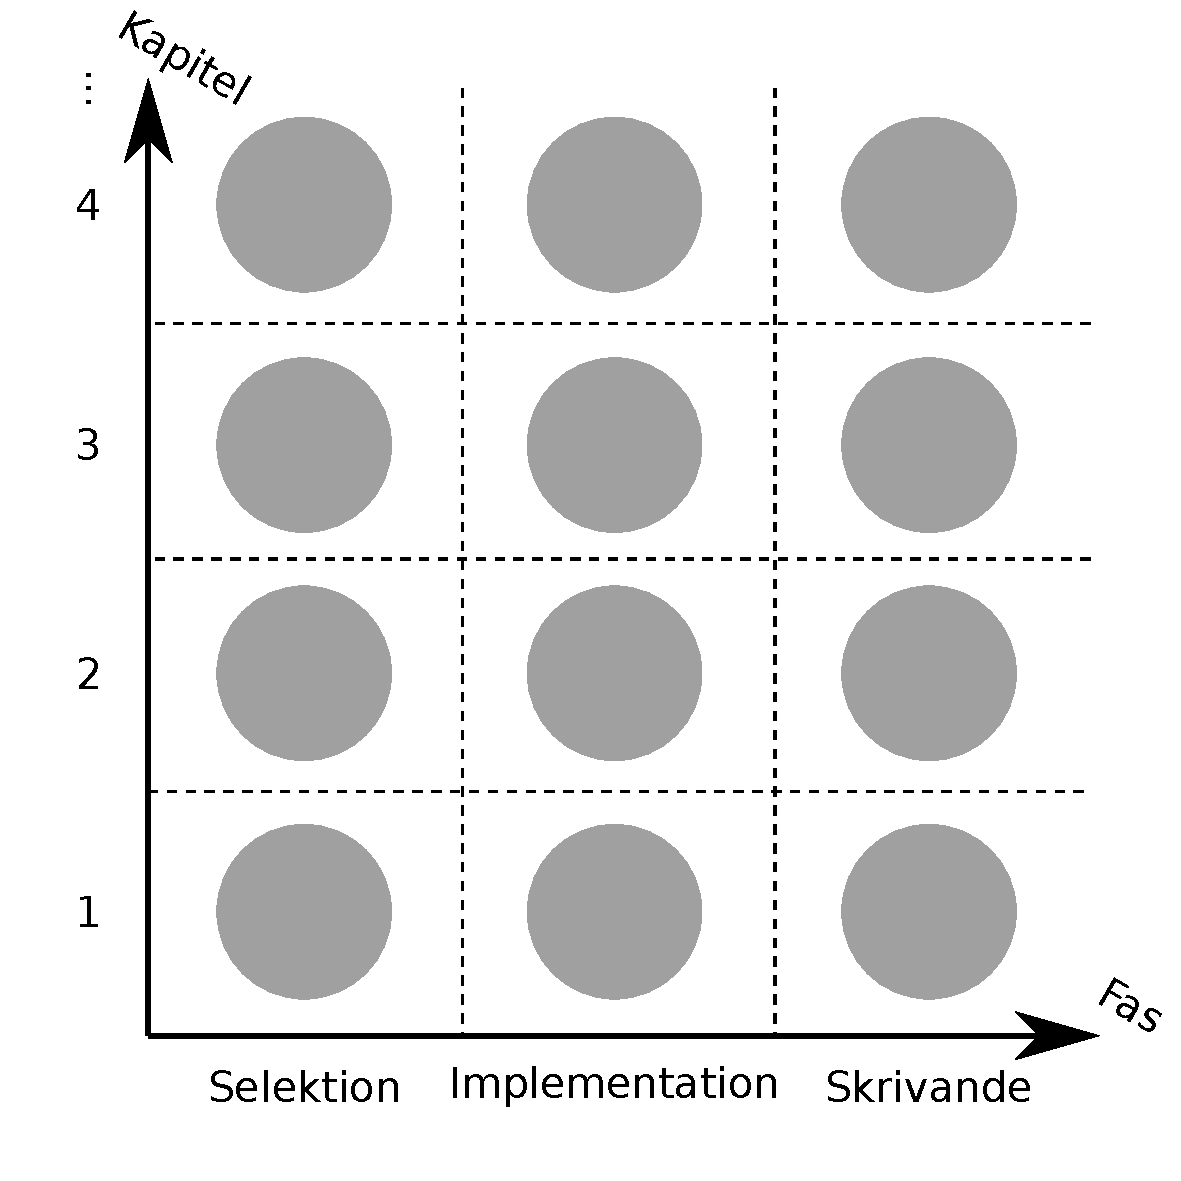
\includegraphics[width=0.9\linewidth]{figure/oversiktA.pdf}}
        \caption{Delarna visas distinkta och var för sig.}\label{fig:oversiktA}
    \end{subfigure}% <- This comment makes the figure lie side by side ¯\(°_o)/¯
    ~~~
    \begin{subfigure}[t]{0.5\textwidth}
        \centering
        \frame{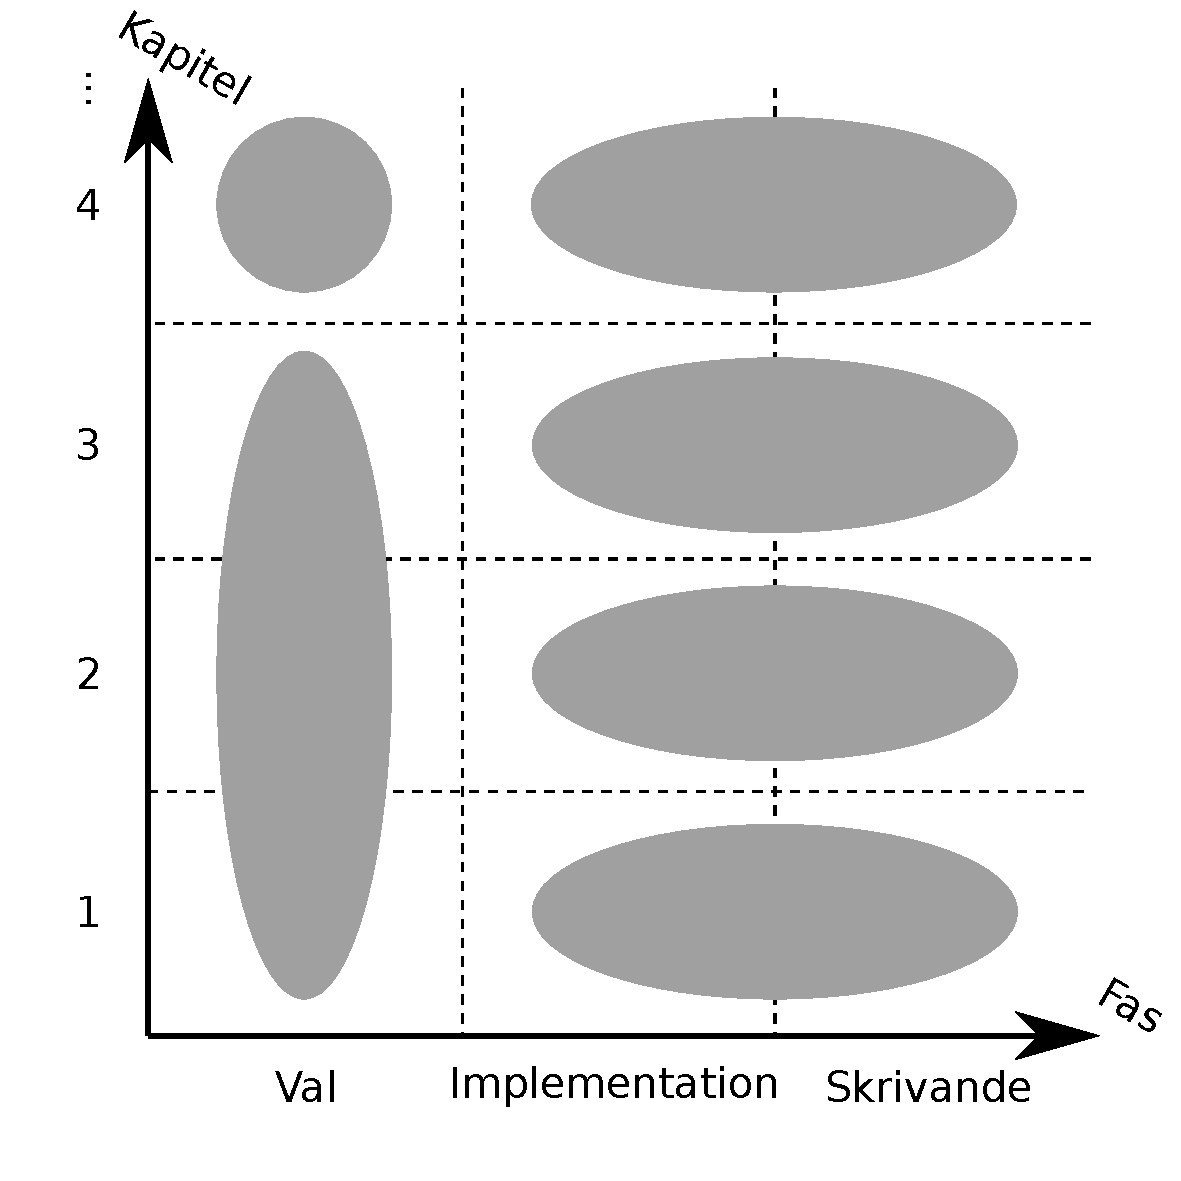
\includegraphics[width=0.9\linewidth]{figure/oversiktB.pdf}}
        \caption{Delarna visas med gränsöverskridande överlapp. Notera att
        implementation och skrivande \textit{alltid} var överlappande medan
      sökande \textit{ofta men inte alltid} var det.}~\label{fig:oversiktB}
    \end{subfigure}
    \caption{Översikt över hur skapandeprocessen av läromaterialet såg ut.
  Processen delas upp utefter två axlar: kapitel och fas. Varje kombination
  är en del som arbetats med och är gråmarkerad.} 
\end{figure}

Även om detta sätt att dela upp processen är översiktlig är den inte helt
verklighetstrogen. I praktiken fanns det överlapp mellan de olika delarna, både
med avseende på kapitel och fas. Det här illustereras i
figur~\ref{fig:oversiktB}. Där ser man att sökandet av områden skedde för flera
kapitel samtidigt. Detta då arbetet med att hitta ett områden ofta gav flera
områden samtidigt. I figuren ser man också att implementation av domänspecifika
språk och skrivande av lärotext skedde samtidigt. Eftersom de i resultatet är
sammanvävda var det också högst naturligt att processerna med att skapa dem
även de var sammanvävda.

Genom hela projektet har skapande av kapitlena skett parallellt. De olika processerna har även befunnit sig i olika faser samtidigt.

De tre följande avsnitten beskriver i detalj hur de tre faserna, val, implementation och skrivande, såg ut. Det är viktigt att minnas att det, som nämndes ovan, fanns överlapp mellan både faserna och kapitlena.

\subsection{Sökande efter områden att behandla}\label{sec:valet}

Ett domänspecifikt språk modellerar ett specifikt och avgränsat område. Därför var det naturligt att söka och tänka i termer av avgränsade områden inom fysiken. För att rent praktiskt hitta områden att behandla kontaktades Åke Fäldt, examinator för Fysik för ingenjörer\cite{tif085} och dess bok (University Physics\cite{UP}) och övrig material studerades.

Denna sökandeprocess innefattade inte bara att \textit{hitta} fysikaliska områden utan även \textit{organisera} dem i relation till varandra. Som framgår senare är till exempel vissa områden påbyggningar av andra. Denna organisering var viktig för att kunna implementera de domänspecifika spårken på bästa sätt och undvika överlappande implementationer.

\subsubsection{Kontakt med Fäldt}
\label{sec:kontakt_faldt}

Fäldt befrågades om vilka områden han i allmänhet anser studenter har
svårt för. Detta för att i enlighet med projektets mål börja med de, för
studenterna, problematiska områdena. Enligt Fäldt är ett allmänt problem att
egna mentala modeller för problem är felaktiga eftersom studenter ofta tar
genvägar som inte bygger på saker de är säkra gäller. En annan erfarenhet
från honom är att så länge första raden i en uppgiftslösning är rätt, så är
resten också rätt. Med andra ord, har studenten väl identifierat vilken typ av
problem det rör sig om brukar det inte vara några svårigheter att lösa
uppgiften.

Med hjälp av insikterna från Fäldt drogs två slutsatser. Den första slutsatsen
var att matematisk analys var ett område värt att behandla i detalj. Den andra
slutsatsen var att genom att ge struktur till olika typer av problem skulle det
förhoppningsvis kunna underlätta för studenter att lära sig att identifiera vilken
typ av uppgift de handskas med.

\subsubsection{Studerande av kursbok och kursmaterial}

Efter kontakten med Fäldt kunde ett sökande efter konkreta områden genomföras. Detta gjordes genom att studera kursboken och kursmaterialet tillhörande Fysik för ingenjörer. Innehållet som hittades delades upp i avgränsade områden för att de skulle bli lämpade till varsitt domänspecifikt språk. Speciellt av intresse var de kapitel som behandlade mekanik (i enlighet med projektets mål att börja med klassisk mekanik), matematisk analys samt de kapitel som använde sig av en specifik syntax \todo{Syntax?}. Domänspecifik syntax var av intresse att finna då en betydlig del av domänspecifika språk är modellering av just syntaxen. \todo{Kanske förtydliga/utveckla varför detta är av intresse}

Sökandet i kursboken och kursmaterialet gav viktiga kunskaper om områden att behandla. Men minst lika viktiga var de inledande experiment som gjordes på varje område för att se huruvida det lämpade sig att göra ett domänspecifikt språk av och hur det skulle kunna se ut. Experimenten visade att enbart vissa områden, till exempel vektorer, fungerade bra att göra ett domänspecifikt språk av. Andra områden, till exempel lutande plan, var mindre lämpliga. Förenklat sagt var enbart områden med tydlig data och tydliga operationer lämpade. Detta diskuteras utförligare i avsnitt \ref{sec:lampligt}. Det framgick också att det blev överlapp mellan olika domänspecika språk trots att områdena var fristående. Ett exempel var det domänspecifika språk för partiklar som till stor del liknade de domänspecifika språken för matematisk analys och vektorer.

Det blev av dessa skäl nödvändigt att göra en distinktion mellan två typer av områden: \textit{grundläggande} och \textit{komposita}. Grundläggande områden är helt fristående från andra områden och behandlar grundläggande koncept. Komposita områden bygger vidare på andra områden eller tillämpar andra områden på konkreta fysikaliska problem.

\subsubsection{Områden som valdes ut}

TODO: Skriv om att varför just dessa. Var för att projektgruppen identifierade dessa grundläggande områden som resten av fysiken byggde på.

De grundläggande områdena som under projekets gång valdes ut blev bevis, dimensioner, matematisk analys och vektorer.

När kunskap inhämtats om olika områden kunde ett urval göras. De områden som identifierades som grundläggande och hade en väl lämpad struktur (se avsnitt \ref{sec:valdes lampligt}) ut. Med detta som grund blev följande de områden som valdes ut.

\textbf{OCH FLER?}

\textit{Bevis} eftersom det ger en insikt i hur de formler man använder
faktiskt uppstår. För att genomföra bevis krävs också att formler och
beteckningar görs rigorösa, vilket ger en bättre förståelse av dem.

\textit{Dimensioner} eftersom det är viktigt för studenter att förstå sig på
hur dimensioner påverkas av algebraiska operationer. Det kan också vara
hjälpsamt att kunna utföra automatisk, datorassisterad dimensionsanalys på
beräkningar.

\textit{Matematisk analys} eftersom alla koncept i klassisk mekanik är
relaterade genom matematisk analys. Mer specifikt används differenser för att
beskriva medelrörelse, och infinitesimalkalkyl för att beskriva
momentanrörelser. Vidare var infinitesimalkalkyl just det område som Fäldt
pekade ut som speciellt viktigt och något som studenter har svårt för.

\textit{Vektorer} eftersom det är en viktig grundsten inom den klassiska
mekaniken. Alla krafter, hastigheter och accelerationer betraktas som vektorer i
planet eller rummet, och dessa är alla fundamentala element inom klassisk
mekanik.

\end{draft}
\begin{binge}

TODO: Skriv om varför just dessa komposita. Finns säkert många komposita, så något urval måste ha gjorts.

De komposita som valdes ut blev...

Ett exempel på ett komposit område är momentan- och medel-rörelse eftersom det
direkt utgör en stor delmängd av alla problem inom mekanik i Fysik för
ingenjörer. Väldigt många av de uppgifter studenter lär sig lösa inom mekanik
är sträcka/hastighet/acceleration/kraft problem. Hur lång tid tar det att åka
en sträcka om man har en viss medelhastighet? Om ett objekt med massa $m$
påverkas av en kraft som varierar enligt $\sin(t)$, vad är då
momentanhastigheten vid $t=10$? Detta är en kombination av det grundläggande
området som behandlar vektorer och området som behandlar matematisk analys.

\end{binge}
\begin{draft}

\subsection{Implementation av DSL för områdena}

Implementationen av ett domänspecifikt språk till ett område inleddes med att
bygga vidare på den experimentering som gjorts under urvalsfsen. Det finns inte
ett rätt sätt att skriva ett domänspecifikt språk på, därav gjordes försök med
flera olika varianter för att se vad som fungerade bäst. Implementationen var en
iterativ process. I flera fall har implementationer gjorts om från grunden om
det visat sig först en bit in att implementationen kunde gjorts bättre eller
hade brister. Dessutom gjordes, i varierande mån, inläsning av domänspecifika
språk, fysik och Haskell för att kunna implementera på bästa sätt.

Vad som ansågs vara en bra, eller åtminstone tillräckligt bra, implementation
var i huvudsak baserat på gruppmedlemmarnas intuition om Haskell och diskussion
inom gruppen och med handledaren. Det viktigaste var att de skulle vara
lättförståliga. Den progamtekniskt elegantaste implementationen användes därför
inte alltid, utan den mer verbosa versionen föredrogs för att göra
läromaterialet så lättläst som möjligt. Dock avstods det inte från använding av
mer avancerade funktioner i Haskell när de var motiverade av materialet som
beskrevs, men då alltid med en utömmande förklaring av hur det fungerade och
utan krav på tidigare kunskap hos läsaren.

Efter att ett domänspecifikt språk implementerats skrevs tester till det. Det
som var intressant att testa var olika lagar som skulle gälla. Eftersom de
domänspecifika språk modellerade matematik var det matematiska lagar som skulle
gälla. Ett exempel var att vektoraddition skulle vara kommutativ. Testerna
gjordes med hjälp av \textit{QuickCheck}. QuickCheck är ett testningsverktyg i
Haskell som genererar många och slumpmässiga testfall. Att lagarna gällde för de
domänspecifika språken verifierades med andra ord genom testa för många
exempelvärden. Inga bevis av att lagarna gällde gjordes.

\subsubsection{Implementation av grundläggande områden}
\label{sec:grund_impl}

För att konkret visa hur en implementationen av ett grundläggande område ser ut
och motiveringen bakom den visas här ett exempel. Exemplet kommer från
läromaterialet och implementerar fysikaliska dimensioner i Haskell.

I fysiken finns det dimensioner \cite{dimensioner_ne}. Några exempel är \textit{längd},
\textit{hastighet} och \textit{massa}. Dimensionerna kan läggas i en av två
kategorier: basdimensioner eller sammansatta dimensioner. Det finns enbart sju 
basdimensioner (längd, massa, tid, elektrisk ström, temperatur, substansmängd och
ljusstyrka) medan det finns oändligt många sammansatta. Sammansatta
dimensioner fås genom att multiplicera eller dividera två andra dimesnioner. Av
de tre exempelna är den första och sista basdimensioner, medan den sista är
sammansatt.

En första ansats till implementation skulle därför kunna se ut som

% Dessa inställningar ska bara användas vid "inline" kod som ej är separat figur.
\begin{lstlisting}[frame=none, belowskip=-0.5\baselineskip, xleftmargin=0.5in]
 data BD        -- Basdimension
        = Le    -- `Längd'
        | Ma    -- Massa
        | Ti    -- Tid
        | Cu    -- `Eletrisk ström'
        | Te    -- Temperatur
        | Su    -- Substansmangd
        | Lu    -- Ljusstyrka
\end{lstlisting}

där \texttt{BD} syntaktiskt representerar de sju basdimensionerna.
Sammansatta dimensioner kan representeras med följande syntaxträd

\begin{lstlisting}[frame=none, belowskip=-0.5\baselineskip, xleftmargin=0.5in]
data Dim = BaseDim BD   -- `Löv med grundläggande dimension'
         | Mul Dim Dim  -- `Förgrening med multiplikation mellan två andra dimensioner'
         | Div Dim Dim  -- `Förgrening med division mellan två andra dimensioner'
\end{lstlisting}

Några exempelvärden blir då

\begin{lstlisting}[frame=none, belowskip=-0.5\baselineskip, xleftmargin=0.5in]
`length = BaseDim Le'
`velocity = Div length (BaseDim Ti)'
\end{lstlisting}

Denna implementation har dock två problem. För det första finns det en
syntaktisk, men ingen semantisk, skillnad mellan

\begin{lstlisting}[frame=none, belowskip=-0.5\baselineskip, xleftmargin=0.5in]
Le
\end{lstlisting}

och

\begin{lstlisting}[frame=none, belowskip=-0.5\baselineskip, xleftmargin=0.5in]
BaseDim Le
\end{lstlisting}

För det andra måste olika syntaktiska former kunna förenklas till en och samma
form. Till exempel måste

\begin{lstlisting}[frame=none, belowskip=-0.5\baselineskip, xleftmargin=0.5in]
Mul (Div (BaseDim Le) (BaseDim Ti)) (BaseDim Ti)
\end{lstlisting}

kunna förenklas till

\begin{lstlisting}[frame=none, belowskip=-0.5\baselineskip, xleftmargin=0.5in]
BaseDim Le
\end{lstlisting}

Även om en sådan förenklare går att göra valdes en annan lösning till
läromaterialet. Nyckeln ligger i att betrakta dimensioner som en multipikation
av basdimensioner med exponenter. Ta till exempel hastighet
\begin{align*}
  \frac{Längd}{Tid} \iff Längd^1 * Tid^{-1}
\end{align*}
Då kan följande representation användas för dimensioner

\begin{lstlisting}[frame=none, belowskip=-0.5\baselineskip, xleftmargin=0.5in]
data Dim = Dim Int    -- Exponent till `längd'
               Int    -- Exponent till massa
               Int    -- Exponent till tid
               Int    -- Exponent till `ström'
               Int    -- Exponent till temperatur
               Int    -- Exponent till `substansmängd'
               Int    -- Exponent till ljusstyrka
\end{lstlisting}

Datatypen har sju fält som vardera anger vilken exponent respektive
basdimension ska ha. Värdet för hastighet är

\begin{lstlisting}[frame=none, belowskip=-0.5\baselineskip, xleftmargin=0.5in]
hastighet = Dim 1 0 -1 0 0 0 0
\end{lstlisting}

som har $1$ som exponent för basdimensionen längd och $-1$ som exponent för
basdimensionen tid.

Multiplikation av två dimensioner går till som multiplikation mellan två tal.
Till exempel \begin{align*}
  Hastighet * Tid = (Längd^1 * Tid^{-1}) * Tid^1 = Längd^1 * Tid^{-1 + 1} =
  Längd \end{align*}
Det vill säga, potensregeln används för att beräkna den nya produkten.

Multiplikation mellan två dimensioner i läromaterialet implemtentarades på ett
motsvarande sätt

\begin{lstlisting}[frame=none, belowskip=-0.5\baselineskip, xleftmargin=0.5in]
mulDim :: Dim -> Dim -> Dim
mulDim (Dim le1 ma1 ti1 cu1 te1 su1 lu1) (Dim le2 ma2 ti2 cu2 te2 su2 lu2) =
  Dim (le1+le2) (ma1+ma2) (ti1+ti2) (cu1+cu2) (te1+t2) (su1+su2) (lu1+lu2)
\end{lstlisting}

Expontenterna hos de två dimensionerna som multipliceras adderas i enlighet med
potensregeln.

För att se alla implementationer hänvisas till läromaterialet i sig. Ett utdrag
finns i bilaga \ref{cha:utdrag} och det fullständiga finns tillgängligt på internet \cite{LYAP}.

\subsubsection{Implementation av komposita områden}

Implementationen av komposita områden var en vidareutveckling på de redan
implementerade grundläggande områdena. Detta utfördes genom att kombinera
element från två eller flera områden för att på så sätt tillsammans skapa ett
helt nytt område. Denna kombination växte fram organiskt genom att studera det
områden som skulle implementeras och se vilka av de grundläggande områdena som
låg till grund. Efter en sådan studie växte den faktiska implementationen fram
genom experimentering och diskussion inom gruppen.

Ett exempel på ett komposit område är implementationen av fysik för partiklar
där det grundläggande området vektorer och området om matematisk analys
kombinerades. Anledningen till detta var att partiklars position, hastighet och
acceleration modelleras med vektorer, dessutom är de krafter som påverkar
partiklar även modellerade som vektorer. Sen används matematisk analys för att
göra dessa beräkningar. Därför var det naturligt att modellera klassisk mekanik
med hjälp av vektorer vars komponenter var datatypen för uttryck som
implementerades av matematisk analys.

Exempel från läromaterialet:
\begin{lstlisting}[frame=none, belowskip=-0.5\baselineskip, xleftmargin=0.5in]
type Mass    = FunExpr
type VectorE = Vector3 FunExpr -- Vector of functional expressions

data Particle  = P { pos  :: VectorE -- Position as a function of time, unit m
                   , mass :: Mass   -- Mass, unit kg
                   }
\end{lstlisting}

\subsection{Skriva lärotext}

I samband med att ett område implementerades skrevs också den tillhörande
lärotexten. Till en början skrevs lärotext som fokuserade på att förklara
programkoden. Detta var ett naturligt val eftersom det var viktigt att
programkoden gick att förstå innan kopplingar till matematik och fysik kunde
förklaras. Det var nämligen lärotext av det slaget som skrevs senare.
Avslutningsvis skrevs inledning och avslutning till kapitlet.

Generellt under skrivningen togs det hänsyn till en specifik underaspekt i ARCS-modellen, nämligen \textit{humor}. Språket i lärotexten har varit lättsamt, vardagligt och talspråkligt för att hålla kvar uppmärksamheten hos läsaren. Det har även ritats roliga bilder för att ge ytterligare humoristiska drag.

Lärotexten och programkoden skrevs sammanvävt i samma fil, i Literate
Haskell. Literat programmering passade bra ihop med
hur läromaterialet skulle se ut då det betonade det jämnbördiga förhållandet
mellan programkod och förklaringar. För att läromaterialet skulle vara
lättförståeligt var det också viktigt att presentera materialet i den ordning
som en mänsklig läsare, och inte datorn, tyckte var enklast. Avsnitt \ref{sec:lhs} beskriver hur literat programmering fungerar i allmänhet och ger
en bra bild hur det såg ut även i detta projekt.

Under skrivandet av lärotexten passades övningar på att läggas till. Oftast
skapades övningar genom att befintlig lärotext modifierades till att istället
för att bara förklara allt, då och då uppmana läsaren att göra nästa steg i
implementationen själv. Nästa steg behölls alltid för att fungera som facit. När
ett kapitel var avslutat lades dessutom extra övningar till i slutet. Dessa
övningar var ofta vidareutvecklingsmöjligheter av det domänspecifika språk som
fanns.

Skrivandet av lärotexten till de grundläggande och komposita områden var
övergripande likadana. Skillnaden låg i balansen mellan Haskell och fysik. För
de grundläggande områdena fokuserade lärotexten mer på Haskell eftersom det var
ett domänspecifikt språk som skulle konstrueras. Hur det fungerade var därför
viktigt att förklara. Dessutom var de fysikaliska och matematiska inslagen inte
alltför stora. I kontrast står lärotexten för det komposita områdena, där ett
större fokus låg på fysik. För dessa områden visades hur de domänspecifika
språken var praktiskt användbara och då förklarades fysik, för att sedan kunna
visa hur den fysiken kunde represententeras i de domänspecifika språken.

Ett exempel på ovanstående är kapitlet kring det komposita området om fysik för
partiklar. Dess implementation var en sammanslagning av området vektorer och
matematisk analys, där istället för att visa och förklara hur områdena kunde
implementeras i Haskell visade hur det direkt gick att översätta de
fysikaliska formlerna som beskriver partiklars rörelse och energier till
Haskell-kod med hjälp av de grundläggande områdena. Beskrivning av relationen arbete-energi (engelska Work-Energy theorem) gick då till som i figur \ref{fig:komposit-ex}:

\begin{figure}[tph]
  \centering
  \fbox{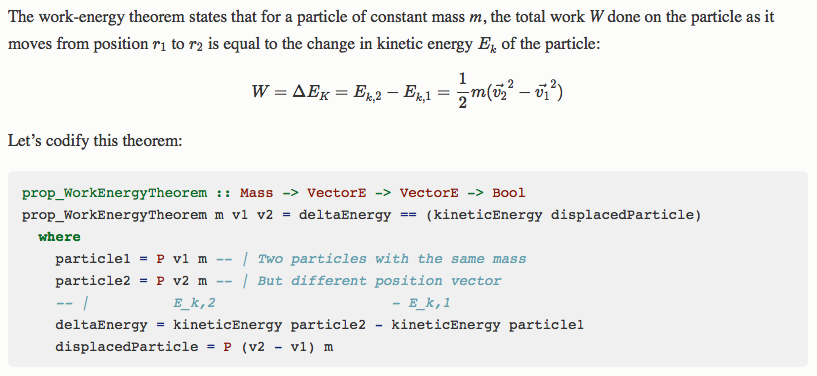
\includegraphics[width=1\textwidth]{figure/komposit-Ex.png}}
  \caption{Implementation av relationen arbete-energi i läromaterialet}
  \label{fig:komposit-ex}
\end{figure}

Implementation kan kompileras och testas och ska då visa på att
implementationerna av de grundlägganden områdena är både rigorösa och korrekta.
Dessutom visar det att går att använda det material som presenteras tidigare
till  att implementera och lösa mer komplexa problem.

\end{draft}
\begin{draft}

\section{Skapande av och publicering på hemsidan}

Läromaterialet kompilerades med hjälp av ett bygg-script och
publicerades på en internethemsida. Bygg-scriptet anropar
\textit{Pandoc} för att konvertera från källkod och text i Literate
Haskell format till HTML, redo att visas på en hemsida. Pandoc
packeterar även med \textit{MathJax} som använder JavaScript för att
rendera matematiska formler i LaTeX format på fint och läsbart
vis. Utan stöd för JavaScript skrivs matematik ut som omodifierad
LaTeX kod, vilket är mer svårläst, men fortfarande tolkningsbart. Det
skrevs även \textit{CSS} manuellt för att modifiera utseendet av
hemsidan sådant att den blev mer fin och läsbar enligt
projektmedlemmarna.

Varje källfil betraktades som ett kapitel och publicerades som
separata undersidor. Med hjälp av ett index beskrivet i bygg-scriptet
konstruerades navigationselement mellan kapitel på varje undersida
och en innehållsförteckning.

För publicering lades all data producerad av bygg-scriptet i en ny git
branch med namnet \texttt{gh-pages}. Att alla branches synkroniseras
mot GitHub medför att alla filer på \texttt{gh-pages} branchen
serveras som en hemsida med hjälp av \textit{GitHub
  Pages}. Publiceringen skedde inte kontinuerligt eller automatiskt,
utan krävde en manuell synkronisering vid varje önskad uppdatering av
hemsidan.

\end{draft}
\begin{draft}

\section{Utvärdering med testgrupp}

  % Återkoppling från examinator (NAD): "Nils Anders Danielsson <nad@cse.gu.se>
  % 27 Feb (1 day ago)
  % to Patrik, Andreas
  % Hi,Your BSc project groups both try to make tools for learning. I had some
  % discussion with Andreas' group about their plans for evaluating how well
  % their product works. My position is that, given the resource limits of
  % these projects (and general problems of reproducibility in social
  % sciences), it is very hard to perform an evaluation that gives useful
  % results. I don't mind if your groups try to perform some kind of
  % evaluation, but I suggest that you tell them to avoid overstating the
  % importance of the evaluations in the final reports."
  % Jag tror det är kompatibelt med det jag sagt tidigare - att göra en "ordentlig" utvärdering av det pedagogiska utfallet är komplicerat och tar (kalender-)tid.
  % Informell utvärdering av en testgrupp bör dock ingå.

För att utvärdera läromaterialet gjordes en kort och informell utvärdering med en testgrupp. Testgruppen bestod av tre andra studenter på Chalmers som gick tredje året på Datateknik eller Informationsteknik. De hade alla läst Fysik för ingenjörer eller motsvarande sedan innan och de hade läst en kurs i Haskell. Däremot hade de inte läst DSLsofMath eller motsvarande. Domänspecifika spårk var med andra ord nytt för dem.

Utvärderingen gjordes genom att visa dem läromaterialet och ge det en kort presentation och bakgrund. Sedan fick de på egen hand läsa det. Deras spontana reaktioner och svar på frågor noterades.

\section{Möten med Fäldt}

För att få återkoppling på läromaterialet hölls två möten med Åke Fäldt, föreläsare och examinator för Fysik för ingenjörer. Ett möte hölls relativt tidigt i projektets skede, 2018-03-02, och ett andra relativt sent, 2018-04-11. Under mötena presenterades läromaterialet i sig och tanken med det, nämligen att presentera fysik på ur ett annat perspektiv, ett funktionellt programmeringsperspektiv. Det diskuterades också svåra områden i Fysik för ingenjörer, vad läromaterialet skulle kunna bidra med för kunskaper till studenter samt dess eventuella roll i relation till fysikkursen i övrigt.

Fäldt befrågades även på vilka fysikalsika områden datastudenter haft svårt för i Fysik för ingenjörer. Detta finns beskrivit i avsnitt \ref{sec:kontakt_faldt}.

\end{draft}


























\chapter{Resultat}

I detta kapitel redovisas det resulterande läromaterialet, vilket består av fem
kapitel. Det är publicerat på en hemsida och dess källkod är fritt tillgänglig.
Även resultaten från utvärderingen med testgruppen och mötena med Åke Fäldt
redovisas.

\section{Läromaterialet}\label{sec:res_laromaterial}

Detta avsnitt innehåller en översikt av läromaterialet samt ett axplock av innehållet ur
vardera kapitel. Axplocken exemplifier delar av läromaterialet och
implementationerna av de domänspecifika språken. De fullständiga implementationerna
är inte inkluderade (och förklarade) eftersom det är precis det läromaterialet
innehåller. Rapporten skulle då bli en kopia av läromaterialet. Istället
finns ett längre utdrag i bilaga~\ref{cha:utdrag} samt hemsidan där
läromaterialet~\cite{LYAP} finns tillgängligt. De avsnitt i rapporten som beskriver läromaterialets innehåll är inga
exakta kopior ord-för-ord utan de har anpassats till
rapporten.

\subsection{Översikt}

Läromaterialet är en löpande text där Haskell-kod och lärotext sammanvävts. Det
ser ut som i figur~\ref{fig:smakprov_laromaterial}. Lärotexten förklarar både fysik, Haskell och hur de relaterar till varandra. I texten följer läsaren med
i implementationen av ett domänspecifikt språk och det visas hur det används.
Tanken är att läsaren parallellt programmerar det som texten förklarar, för att
på så sätt även få praktisk färdighet i det som presenterats. För detta syfte
finns det även övningar tillagda direkt i den löpande texten, se
figur~\ref{fig:smakprov_ovning}, som ofta innebär att läsaren själv ska
implementera en liten del av det domänspecifika språket. Det finns också
övningar i slutet av kapitlet som ofta innebär större vidareutvecklingar av de
domänspecifika språken.

\begin{figure}[h]
    \centering
    \begin{subfigure}[t]{0.5\textwidth}
        \centering
        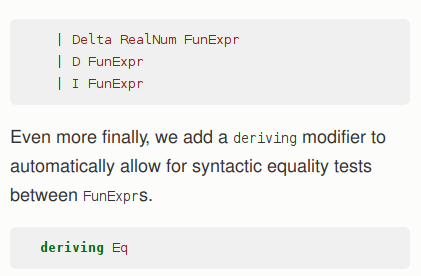
\includegraphics[width=0.9\linewidth]{figure/smakprov_laromaterial.png}
        \caption{Lärotexten är mot den ljusgrå bakgrunden medan Haskell-kod är mot den mörkgrå.}~\label{fig:smakprov_laromaterial}
    \end{subfigure}%
    ~~~
    \begin{subfigure}[t]{0.5\textwidth}
        \centering
        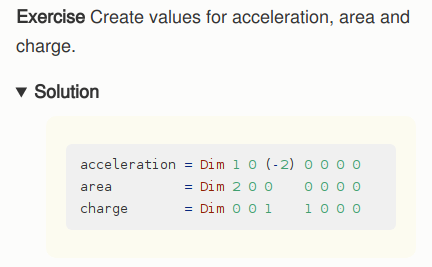
\includegraphics[width=0.9\linewidth]{figure/smakprov_ovning.png}
        \caption{Exempel på en övning. Övningen ligger som en del av den
                 löpande texten.}~\label{fig:smakprov_ovning}
    \end{subfigure}
    \caption{Ett smakprov av det resulterande läromaterialet.}
\end{figure}

Språket i lärotexten är enligt projektgruppen lättsamt\footnote{Diskuteras
utförligare i avsnitt \ref{sec:res_disk}.} och i detta syfte finns det även
bilder tillagda. Figur~\ref{fig:smakprov_bild_laromaterial} är ett exempel på en
bild ur läromaterialet. Notera speciellt den medvetet oseriösa ritningstekniken
som är tänkt att vara rolig och muntra upp läsaren.\newline

% newline ska kanske bort. Är för formatering

\begin{figure}[h]
        \centering
        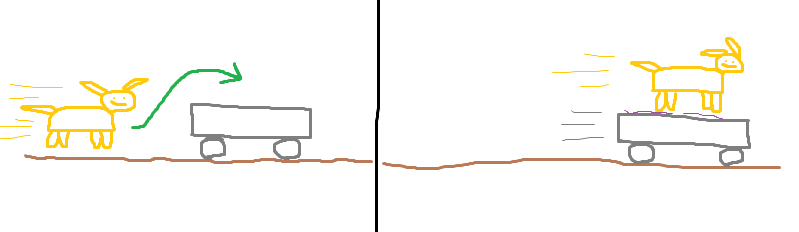
\includegraphics[width=0.4\linewidth]{figure/smakprov_bild_laromaterial.png}
        \caption{Exempel på en bild. Bilden visar hur en hund springer och hoppar upp på en stillastående vagn.}
        \label{fig:smakprov_bild_laromaterial}
\end{figure}

Läromaterialet innehåller fem kapitel som vardera behandlar ett område inom fysik
och matematik. Fokuset är på klassisk mekanik samt den matematik som tillhör
området. De behandlade områdena är:

\begin{itemize}
  \item Dimensioner
  \item Matematisk analys
  \item Vektorer
  \item Exempelproblem
  \item Partikelmekanik
\end{itemize}

\textit{Dimensioner} behandlar fysikaliska dimensioner, storheter och enheter inom fysiken.
Fysikaliska dimensioner införs på typnivå i Haskell för att visa likheten mellan
Haskells typsystem och hur dimensioner hanteras inom fysiken.
Typnivåprogrammering\footnote{Vanligtvis manipuleras \textit{värden} när
programmerering sker i Haskell och andra språk. Typnivåprogrammering är precis som
vanlig programmering med skillnaden att den sker på typnivån, det vill säga, att
typer modifieras. För en utförligare förklaring av typnivåprogrammering, se läromaterialet~\cite{LYAP}.} används för att göra likheterna så tydliga som möjligt.

I \textit{matematisk analys} behandlas differentialkalkyl och
integralkalkyl för en variabel. Först bestäms den semantiska domänen
för analys i en variabel: reella funktioner av ett argument; och ett syntaxträd
för uttryck av funktioner inom denna domän konstrueras. Därefter
analyseras syntax och semantik för differenser, derivator, och
integraler; och funktioner implementeras för att utföra dessa
operationer både approximativt numeriskt, och symboliskt med ett
syntaxträd. Slutligen appliceras de implementerade funktionerna för
att visualisera grafer av operationerna.

\textit{Vektorer} behandlar vektorer och vektoroperationer. Vektorer modelleras
med hjälp av en typklass som dikterar vilka funktioner som varje
modell av en vektor måste implementera. Generella vektoroperationer såsom
addition och skalärprodukt implementeras sedan med hjälp av dessa funktioner
vilket skapade ett mycket generellt och lättanvänt gränssnitt. QuickCheck
användes för att verifiera lagarna som gäller för olika vektoroperationer,
vilket gav en generell säkerhet kring att implementationerna var korrekta.

I \textit{exempelproblem} tillämpas de tre tidigare kapitlen på två vanliga
mekanikproblem, nämligen \textit{krafter på lådor} och \textit{gungbräda}. I
krafter på lådor används det domänspecifika språket för vektorer till att
beräkna de krafter som verkar på en låda som glider ner för ett plan. I
gungbräda visas hur momentjämviktsberäkningar kan göras med det domänspecifika
språket för dimensioner.

\textit{Partikelmekanik}. En repetition av gymnasieskolans fysik.
Lägesenergi, rörelseenergi, gravitation och så vidare. Den modelleras med vektorer vars
komponenter består av matematiska uttryck tagna från kapitlet om matematisk
analys. Förhoppningen är att detta område inte ska presentera någon ny fysik för
läsaren utan istället visa hur redan känd fysik direkt går att översätta till
läromaterialets domänspecifika språk.

Läromaterialet blev publicerat på en hemsida~\cite{LYAP} och all källkod finns
tillgänglig på projektets GitHub~\cite{LYAP_repo}. På GitHub finns även ett
antal delvis färdigställda områden, till exempel bevisföring. Texten i
läromaterialet är skriven på engelska.

\subsection{Dimensioner}
\label{sec:grund_impl}
\label{sec:res_dim}

I detta avsnitt visas delar av hur implementationen av dimensioner ser ut i
läromaterialet. Den fullständiga implementationen innehåller tre delar:

\begin{enumerate}
  \item Dimensioner på värdenivå
  \item Dimensioner på typnivå
  \item Datatyp för storheter
\end{enumerate}

Dimensioner på värdenivå används för att enkelt kunna skriva ut dimensioner i
GHCi. Dimensioner på typnivå används för att ge typsäkerhet till dimensioner, så
att till exempel en längd och en massa inte kan adderas, likt att ett värde av
typ \texttt{Double} och \texttt{Integer} inte kan adderas i Haskell. Till sist
kombineras de två varianterna av dimensioner till en datatyp för storheter som
aritmetiska operationer kan utföras på.

Dimensioner kan ses som en produkt av de 7 basdimensionerna\footnote{Längd,
massa, tid, elektrisk ström, temperatur, substansmängd och ljusstyrka.}, med en
indiviudell exponent till varje basdimension. Datatypen, på värdenivå, som
används ser därför ut som följande

\begin{lstlisting}
data Dim = Dim Integer -- Length
               Integer -- Mass
               Integer -- Time
               Integer -- Current
               Integer -- Temperature
               Integer -- Substance
               Integer -- Luminosity
    deriving (Eq)
\end{lstlisting}

Varje fält i datatypen representerar exponenten för motsvarande basdimension. Om
exponenten är $0$ betyder det att den basdimension inte är inkluderad i
dimensionen. Några exempel ges för att förtydliga.

\begin{lstlisting}
length      = Dim 1 0 0 0 0 0 0
mass        = Dim 0 1 0 0 0 0 0
time        = Dim 0 0 1 0 0 0 0

velocity     = Dim 1 0 (-1) 0 0 0 0
acceleration = Dim 1 0 (-1) 0 0 0 0
area         = Dim 2 0   0  0 0 0 0
\end{lstlisting}

Hastighet skrivs vanligtvis som $\frac{m}{s}$ men ekvivalent är att skriva
$m^1*s^{-1}$ vilket förklarar varför värdena ovan ser ut som de gör.

I resterande del av detta kapitel i läromaterialet visas hur multiplikation och
division samt hur en \textit{utskriftsfunktion}, som skriver ut ett värde
snyggt, kan implementeras. Därefter följer ett antal delkapitel som innehåller
testning, typnivådimensioner och storheter.

\subsection{Matematisk analys}

I kapitlet om matematisk analys skapas en syntax för funktionsuttryck och symboliskt derivering och integrering implementeras. Dessutom analyseras syntax och semantik hos uttryck som dyker upp inom matematisk analys, till exempel $\Delta$-operatorn.

Syntaxen för funktionsuttryck inleds med

\begin{lstlisting}
data FunExpr = Exp | Log | Sin | Cos | Asin | Acos
\end{lstlisting}

vilket är ett antal elementära funktioner. Näst följer aritmetiska operationer. För att kunna definera dem på \textit{funktioner} och inte algebraiska \textit{uttryck} görs nedanstående tolkning
\begin{align*}
  f \text{ $OP_{r \to r}$ } g = x \mapsto (f(x) \text{ $OP_r$ } g(x))
\end{align*}
vilket utökar \texttt{FunExpr} med fler konstruktorer.

\begin{lstlisting}
    | FunExpr :+ FunExpr
    | FunExpr :- FunExpr
    | FunExpr :* FunExpr
    | FunExpr :/ FunExpr
    | FunExpr :^ FunExpr
\end{lstlisting}

Även konstruktorer för den oberoende variablen, konstanter, funktionskomposition, $\Delta$, derivering och integrering behövs.

\begin{lstlisting}
    | Id
    | Const RealNum
    | FunExpr :. FunExpr
    | Delta RealNum FunExpr
    | D FunExpr
    | I FunExpr
\end{lstlisting}

En utförligare förklaring av syntaxen \texttt{FunExpr} finns i läromaterialet.

I läromaterialet analyseras derivering utförligt med gränsvärden, kvoter och approximativa metoder. Dessutom motiveras och implementeras symbolisk derivering. Den görs med en funktion \texttt{derive} som har ett fall för vardera av konstruktorerna i \texttt{FunExpr}. Några av fallen är

\begin{lstlisting}
  derive (f :* g) = derive f :* g :+ f :* derive g
  derive (f :+ g) = derive f :+ derive g
  derive Exp = Exp
\end{lstlisting}

\subsection{Vektorer}

Kapitlet om vektorer inleds med en genomgång av vektorer och operationer på dem parallellt med att en första implementation till dem skrivs. Implementation ser ut som följer

\begin{lstlisting}
  data Vector2 n = V2 n n
  type Scalar = Double
  type VectorTwo = Vector2 Scalar
  
  magnitude :: VectorTwo -> Scalar
  magnitude (V2 x y) = sqrt (x^2 + y^2)
  
  add :: VectorTwo -> VectorTwo -> VectorTwo
  add (V2 x1 y1) (V2 x2 y2) = V2 (x1 + x2) (y1 + y2)

  dotProd :: VectorTwo -> VectorTwo -> Scalar
  dotProd (V2 ax ay) (V2 bx by) = ax * bx + ay * by
\end{lstlisting}

Eftersom vektorer i tre dimensioner ser snarlik ut leder det till väldigt mycket duplicerad kod. En andra implementation görs därför som är mer generell. Grunden är den nedanstående typklassen

\begin{lstlisting}
class Vector vector where
  vmap     :: (n -> n) -> vector n -> vector n
  vzipWith :: (n -> n -> n) -> vector n -> vector n 
                                        -> vector n
  vfold    :: (n -> n -> n) -> vector n -> n
\end{lstlisting}

som innehåller de tre funktioner som behövs för att genomföra vektoroperationerna \texttt{magnitude}, \texttt{add} och \texttt{dotProd}. De kan nämligen skrivas om enbart med hjälp av de funktioner som finns i typklassen \texttt{Vector} på följande sätt

\begin{lstlisting}
  magnitude :: (Floating n, Vector vec) => vec n -> n
  magnitude = sqrt . vfold (+) . vmap (**2)

  add :: (Num n, Vector vec) => vec n -> vec n -> vec n
  add = vzipWith (+)

  dotProd :: (Num n, Vector vec) => vec n -> vec n -> n
  dotProd v1 v2 = vfold (+) $ vzipWith (*) v1 v2
\end{lstlisting}

Allt som behöver göras för vardera datatyp för vektorer av olika längd är därmed att göra den en \texttt{Vector}-instans. Så här ser det ut för \texttt{Vector2}

\begin{lstlisting}
instance Vector Vector2 where
  vmap     f (V2 x y)            = V2 (f x)    (f y)
  vzipWith f (V2 x y) (V2 x' y') = V2 (f x x') (f y y')
  vfold    f (V2 x y)            = f x y
\end{lstlisting}

Resterande del av vektor-kapitlet behandlar kryssprodukt, vektorlagar och tester av dem.

\subsection{Exempelproblem}

Dessa problem är implementationer eller lösningar på fysikuppgifter som har förekommit på tentamen i Fysik för ingenjörer. De använder de andra modulerna i läromaterialet för att göra beräkningarna (exempelvis dimensionsanalys eller vektoroperationer). Av exempelproblemen finns en gungbräda och en låda på ett lutande plan. Då källkoden för dessa problem endast är menade att lösa den specifika uppgiften, och inte alla varianter på gungbrädor eller lådor på lutande plan, så kan de inte kallas för domänspecifika språk, utan är istället implementationer som använder tidigare domänspecifika språk.

Exemplet med gungbrädan har två massor på gungbräda som befinner sig i jämvikt. Uppgiften är att finna en okänd sträcka mellan en av vikterna och balanspunkten. Exemplet använder dimensionsanalys för att representera hävarmseffekten av de olika massorna. Genom att ställa upp förhållanden och lösa ut den okända sträckan, så går det att beräkna den okända sträckan. Sist görs en säkerhetskontroll där den okända sträckan används för att räkna ut hävarmsmomenten, vilket är den sista kontrolleringen att man inte har gjort några logiska fel.

Exemplet med en låda på ett lutande plan undersöker krafterna på en låda på ett lutande plan, såsom gravitationen, normalkraften från det lutande planet, och resultantkraften, vilka representeras genom vektorer från vektormodulen. Detta exemplet tar både hänsyn till statisk friktion (då lådan befinner sig stillastående) och kinetisk friktion (då lådan befinner sig i rörelse).

\subsection{Partikelmekanik}

Implementationen av partikelmekanik är en kombination av de domänspecifika språken för vektorer och matematisk analys. Anledningen till detta är att partiklars position, hastighet och acceleration modelleras med vektorer, dessutom är de krafter som påverkar partiklar även de modellerade som vektorer. Sedan används matematisk analys för att göra beräkningar på dem. Därför är det naturligt att modellera partikelmekanik med hjälp av vektorer vars komponenter är uttryck som implementeras av matematisk analys.

Datatypen för en partikel är

\begin{lstlisting}
type Mass    = FunExpr
type VectorE = Vector3 FunExpr

data Particle  = P { pos  :: VectorE -- Position as a
                                     -- function of time.
                                     -- Unit m
                   , mass :: Mass    -- Mass. Unit kg
                   }
\end{lstlisting}

Ett exempelvärde är

\begin{lstlisting}
particle :: Particle
particle = P (V3 (3 * Id * Id) (2 * Id) 1) 3
\end{lstlisting}

Eftersom komponenterna i vektorerna är funktionsuttryck är det enkelt att beräkna en partikels hastighet och acceleration.

\begin{lstlisting}
velocity :: Particle -> VectorE
velocity = vmap D . pos

acceleration :: Particle -> VectorE
acceleration = vmap D . velocity
\end{lstlisting}

Det går även att beräkna nettokraften på en partikel med hjälp av Newtons andra lag.

\begin{lstlisting}
type Force = VectorE

force :: Particle -> Force
force p = vmap (* m) a
  where
    m = mass p
    a = acceleration p
\end{lstlisting}

I läromaterialet behandlas även rörelseenergi, lägesenergi, arbete och gravitation.

\section{Utvärderingen med testgruppen}\label{sec:res_test}

Utfallet från utvärderingen med testgruppen var till övervägande del positivt.
Testgruppen tyckte läromaterialet var ett intressant och roligt sätt att
presentera fysik på. De tyckte att bilderna tjänade sitt syfte i att muntra upp
läsaren. \todo{Hade de klarat kursen?}

En poäng som framfördes var att inte börja kapitlen för komplicerat. Istället
tyckte de att det skulle vara bra att börja enkelt, för att kunna hänga med i
både Haskell-koden och fysiken, och därefter behandla ett område mer
detaljerat. Att visa ett kort exempel i Haskell för att sedan låta läsaren själv
göra något liknande var ett förslag.

Utvärderingen var dock för kort för att det skulle framgå huruvida läsaren lärde
sig mest fysik eller mest Haskell. Det framgick heller inte om läromaterialet
uppmuntrade testgruppen att vilja lära sig mer fysik.

\section{Möten med fysikläraren}\label{sec:res_ake}

Åke Fäldt hade en överlag positiv syn på läromaterialet\footnote{Det bör
påpekas att det som är återgivet här självklart är en egen tolkning, och kan ha
missuppfattats, av projektgruppen. Fäldt ska med andra ord inte behöva stå till
svars för vad som står här.}. Fäldt tyckte att det fanns flera saker
läromaterialet kunde bidra med. En av dessa var att läromaterialet ger ett annat
perspektiv på fysiken, ett annat sätt att förklara den med
hjälp av domänspecifika språk. En annan sak var den rigorösitet som
domänspecifika språk leder till, eftersom de domänspecifika språken måste vara
väldefinierade betyder det att alla fysikaliska koncept måste göras entydiga så
att även de blir väldefinierade och följden blir att operationerna på dem
enbart kan göras på det definierade sättet. Dessutom måste dimensionerna stämma, vilket nämndes i avsnitt \ref{sec:res_dim}.
Fäldt menade att det var en bra egenskap hos läromaterialet, att detta rigorösa
tankesätt och metodik som förmedlas hade varit till nytta för problemlösning i
fysikkursen.

Förutom ovanstående framgick även vilka områden i Fysik för ingenjörer som var
svåra för studenter, vilket användes vid sökandet efter områden, se avsnitt \ref{sec:valet}.

\section{Möte med programansvarig och datas nämnd för studier}

Både Roger Johansson, programansvarig på datateknik, och datas nämnd för studier (DNS)
var positiva till projektets initiativ och målsättning. Johansson beskrev
problematiken med att matematiken inte är lika naturlig för datastudenter som för
andra ingenjörsområden.



\chapter{Diskussion}

I detta kapitel diskuteras projektets genomförande, resultat,
vidareutvecklingsmöjligheter och etiska aspekter.

Till att börja med vill vi säga att hur domänspecifika språk kan kombineras med
fysik inte var något vi visste när projektet startade. En stor del av arbetet i
början av projektet ägnades därför åt att försöka komma på olika sätt att
använda dem ihop med olika fysikaliska områden. Det gjordes många experiment
innan vi hittade ett sätt att skapa domänspecifika språk till fysik som var annat än
triviala implementationer av formler, till exempel att formlen för
rörelseenergi, $E_k = \frac{mv^2}{2}$, kan skrivas som \texttt{ek m v = m * v *
v / 2} i Haskell. Detta experimenterande ledde till att
vi kunde se en slags strategi för hur man kan kombinera dem, vilket blev den
metodik som beskrivs i avsnitt~\ref{sec:konstruktion}. Det vi vill poängtera är
med andra ord att det har varit svårt och oklart hur projektet skulle föras
framåt eftersom det inte funnits någon tydlig väg att följa.

\section{Genomförandediskussion}

Under projektets genomförande har det gjorts flera val av teorier och metoder
att använda. Självklart behöver inte dessa val vi gjorde vara de bästa.
Därför kommer vi här att kritisera dem och föreslå andra möjligheter. Närmare
bestämt kommer utvärderingen, urvalet och Literate Haskell att diskuteras.

Utvärderingen som gjordes under projektet kan kritiseras på flera sätt. För det
första bestod testgruppen av enbart tre personer. Fler
personer hade krävts för att få ett mindre snävt underlag. För det andra hölls
utvärderingen under en ytterst kort tid, ungefär en timme. I början av den
timmen såg de läromaterialet för första gången och resterande tid läste
testgruppen igenom det. Utvärderingen hade behövt vara längre för att låta testgruppen
i lugn och ro arbeta igenom ett par kapitel, inklusive att följa med i
programmeringen som gjordes i läromaterialet. För det tredje var vi inte tydliga
med vad för frågor vi ville ha svar på, utan istället noterade vi testgruppens
spontana reaktioner. Vi ville till exempel veta om de tyckte att domänspecifika
språk gav en rigorös struktur till fysik. Men eftersom vi inte gjorde det
tydligt för testgruppen kunde de heller inte tänka på dessa frågor. Med tanke på
dessa tre brister i utvärderingen är alla slutsatser dragna med utvärderingen
som stöd ytterst osäkra.

Det går även att kritisera hur urvalet av områden gick till under projektet.
Dels kan det ha lett till att endast några få domänspecifika språk för fysik
implementerades, se diskussionen i avsnitt~\ref{sec:fpf}. Dels skedde urvalet ur
implementatörens perspektiv (det vill säga, vårt) och inte ur användarens
perspektiv (studenten som ska nyttja läromaterialet). Med det menar vi att
områden valdes utifrån hur det implementationsmässigt hängde ihop, till exempel
att matematisk analys är grunden till flera tillämpningar. Istället hade områden
kunnat väljas utifrån de fysikaliska problem studenter ska lösa i Fysik för
ingenjörer, till exempel lutande plan, block och talja eller momentjämvikt, och
utifrån det utforma domänspecifika språk. De olika sätten att tänka vid val av
områden skiljer sig åt och mest fokus under projektet har lagts på
implementationsperspektivet. Visserligen gjordes enstaka försök att tänka på det
andra sättet också, men vi tyckte det var svårt att skapa några domänspecifika
språk på det sättet (se avsnitt~\ref{sec:lampligt}). Vi hade dock kunnat utforska
detta tankesätt grundligare än vad vi gjort, istället för att avfärda det som
ett svårare sätt att gå till väga.

Till sist kan man kritisera den allmänna metoden som valdes för utformningen av
läromaterialet, nämligen att skriva varje kapitel som en lång, sammanhängande,
löpande text. Lärotexten har skrivits som en berättelse om hur ett
domänspecifikt språk kan implementeras eller tillämpas för olika fysikaliska
områden. Nackdelen är att det blir en passiv inlärning. Läsaren visas hur man
kan göra utan att försöka så mycket själv. Visserligen har övningar inkluderats
i läromaterialet, och läsaren uppmuntras till att implementera koden parallellt, men det
riskerar ändå att bli en passiv inlärning. Valet att använda Literete
Haskell har definitivt bidragit till dessa passiva tendenser. Literate Haskell är
inget annat än en vanlig programfil fast mer väldokumenterad, som i projektets fall varit färdiga implementationer av domänspecifika språk. Det kan till och med vara så att Literate
Haskell är sämre än ``bara'' Haskell, med avseende på aktivt lärande, då det är
enklare att ändra och experimentera med en programfil utan dokumentation som är i vägen. Under
projektets genomförande hade det därför varit av intresse att undersöka
alternativa sätt att utforma lärotexten som uppmuntrat ett mer aktivt lärande.
Det hade till exempel kunnat vara att presentera idén bakom fysikaliska
dimensioner, och sedan låta studenten själv skapa implementationen. Något enkelt
exempel hade kunnat visats först för att ge någon slags fingervisning om hur man
kan göra.

\section{Resultatdiskussion}\label{sec:res_disk}

Detta avsnitt inleds med en övergripande diskussion om det resulterande
läromaterialet, för att sedan övergå till en mer generell diskussion kring
kombinationen av domänspecifika språk och fysik.

I projektets mål och avgränsningar stod det att vi skulle börja med klassisk
mekanik, för att i mån av tid även behandla termodynamik och vågrörelselära. I avsnitt~\ref{sec:res_laromaterial} nämns att de tre grundläggande
områdena dimensioner, matematisk analys och vektorer är färdiga, samt de
komposita områdena partikelmekanik, gungbräda och krafter på lådor. Med andra
ord har mekanik påbörjats, men inte termodynamik eller vågrörelselära. Det som återstår enligt oss när det kommer till mekanik är att tillämpa de grundläggande områdena på
fler fysikaliska problem utöver gungbräda och krafter på lådor. Vi tror att de
tre grundläggande områdena som är färdiga räcker. Förutom fler tillämpningar kan
man utveckla mer fördjupande områden, till exempel bevisföring, något som
nämndes i avsnitt~\ref{sec:res_laromaterial} att det påbörjats. Det är dock värt
att nämna att vi är mycket nöjda med det material som vi har producerat. Våra
kapitel är väl avgränsade, utformade och implementerade på det sätt som vi
anser att de bör.

En annan del av målet var att läromaterialet skulle vara lättillgängligt genom
sitt språkbruk, publicering på en hemsida och fri tillgång till källkoden.
Vi kan konstatera att de senare två har genomförts. Vi passar även på att
säga att vi tycker att en lättanvänd hemsida är trevligare att använda än
PDF-filer eftersom de inte har sidbrytningar, fasta sidmarginaler som använder
skärmutrymme, med mera. Detta är visserligen mindre detaljer, men tillsammans
påverkar de upplevelsen i stort. Vi
tycker även att språket i läromaterialet är någorlunda lättsamt då vi skriver
talspråkligt och vardagligt, och förklarar svårigheterna grundligt. Språket hade
dock kunnat vara vänligare. Till exempel beskriver vi olika koncept som
``väldigt enkla'' fastän läsaren kanske inte alls tycker det.

Vi knyter här även an till lärandeteorierna i avsnitt \ref{sec:arcs}, som nämnde interaktion och snabba belöningar. Vårt läromaterial har visserligen ingen interaktiv sida, men typsystemet i Haskell skulle ändå tänkas kunna fungera som en fingervisare när man gör rätt eller fel. Det går exempelvis inte att räkna med dimensioner på ett felaktigt sätt, och funktionskomposition fungerar endast om båda funktionernas typdefinitioner (typer på argument och returvärde) stämmer överens. När det kommer till snabba belöningar kan den glädje man ser när koden kompilerar ses som en sådan. Läromaterialet innefattar även strategiskt placerade roliga bilder, för att ge impulsiva glädjereaktioner.

Läromaterialet kan vara relevanta för flera grupper. Visserligen är målgruppen datastudenter, och vi har personligen dragit nytta av det,
men vi tror att det kan vara relevant för fler än så, till exempel kan läromaterialet även vara intressant för fysiklärare. Fäldt nämnde att han
tyckte att det rigorösa tankesätt läromaterialet skolar in läsaren i kan vara
användbart även i traditionell fysikundervisning. Det kan därför vara intressant att undersöka hur ett sådant här läromaterial kan
integreras i undervisningen.

En del av projektets mål var att diskutera kombinationen av
domänspecifika språk och fysik. I de tre följande avsnitten diskuterar vi därför
läromaterialets fokus på matematik och Haskell istället för fysik, vilka
fysikaliska områden som var lämpliga att göra domänspecifika språk till samt om
det finns en pedagogisk nytta i att kombinera de två. Diskussionen är till
största del baserad på våra erfarenheter efter att ha implementerat ett flertal
domänspecifika språk relaterade till fysik, men de är även baserade på
uppfattningar från testgruppen och fysikläraren.


\subsection{Om läromaterialets fokus på matematik och Haskell snarare än
fysik}\label{sec:fpf}

Målet med läromaterialet var att lära ut fysik på ett roligt och lättförståeligt
sätt. Dock syns det i resultatet, avsnitt~\ref{sec:res_laromaterial}, att det
stora fokuset lagts på att förklara och lära ut matematik och Haskell. Vi menar att det finns flera anledningar till att ett stort fokus lagts på matematik och Haskell.

Problemet med att prata om en egen implementation av fysik är att fysik inte är
ett helt eget område. Det är snarare så att fysik kan ses som tillämpad
matematik, att fysik använder matematiken för att beskriva det fysikaliska
universum vi lever i. Det blir därför naturligt att när den faktiska
implementationen av dessa beskrivningar och lagar sker, så sker de med hjälp av
matematiken. Det stora fokuset på matematiken är alltså en
konsekvens av fysiken i sig själv. Att fysik är tillämpad matematik illustreras
i figur~\ref{fig:xkcd}, som även visar mer generellt hur en kedja av områdena är
tillämpningar av varandra.

\begin{figure}[tph]
  \centering
  
\includegraphics[width=0.9\textwidth]{figure/purity.png}
  \caption{\href{https://xkcd.com/435/}{Purity} av
  \href{https://xkcd.com}{xkcd.com} licensierad under
\href{https://creativecommons.org/licenses/by-nc/2.5/}{CC BY-NC}. Bilden beskriver hur fysik är en tillämpning av matematik. Det är i själva verket
så att en kedja av områden kan betraktas som tillämpningar av
varandra.}\label{fig:xkcd}
\end{figure}

Självklart ingår det också en stor del problemlösning inom fysik, den faktiska
tillämpningen av de beskrivningar och lagar som matematiken ger oss. Men
problemlösning är något som vi tycker är svårt och problematiskt att modellera
som ett domänspecifikt språk, något som diskuteras djupare i
avsnitt~\ref{sec:lampligt}.

Anledningen till att ett stort fokus läggs på Haskell är att de koncept som används är viktiga för läsaren att förstå. Koncepten är ibland inte kända för en läsare med endast en grundläggande förståelse för Haskell och då måste de förklaras tillräckligt ordentligt för att det ska gå att hänga med. Och
eftersom ett syfte med läromaterialet var att väcka intresse hos läsaren med
bakgrund inom Haskell så ville vi lägga fokus på att tydligt visa
parallellerna mellan funktionell programmering, matematik och implementationen
av fysik.

Vi hävdar alltså att fokuset lagts på mer än bara fysik av två skäl: att fysik är tillämpad matematik och att det är viktigt att förklara de Haskell-koncept som används. Det måste däremot inte vara så. Det kan mycket väl vara så att detta fokusskifte har skett på grund
av hur vi valde att genomföra projektet. I ett tidigt skede valde vi att söka efter
områden som vi ansåg vara fristående och väl avgränsade, se avsnitt~\ref{sec:valet},
och implementera dessa var för sig. Utan tvekan har detta sätt att påbörja
projektet påverkat allting som kom därefter. Om vi istället hade utvecklat
läromaterialet som en kombination av olika områden från början hade det kanske
inte varit lika främmande att även baka in problemlösning i läromaterialet och på så sätt
fått mer fysikorienterade domänspecifika språk.

Men det går det att vara kritisk till projektets utformning redan i ett tidigare
skede. En aspekt är valet av Haskell. Vi hävdar i teorin~\ref{sec:syntax} att
Haskells typer och fokus på mönstermatchning gör det idealt för implementering
av domänspecifika språk, vilket inte nödvändigtvis betyder att det är idealt för implementering av fysik. Det är möjligt att ett objektorienterat språk som Java hade passat bättre. Att
använda ett språk som inte har en lika stark koppling till ren matematik som
Haskell hade kanske lett till att fokuset inte legat på matematiken
bakom fysiken, utan istället på fysiken framför matematiken.

\subsection{Passande områden för domänspecifika språk}\label{sec:lampligt}

Under genomförandet av projektet utfördes flera experiment för att bedöma olika
områdens lämplighet för att modelleras med ett domänspecifikt språk. Det visade
sig snabbt att vissa områden lämpade sig bättre än andra. Områden
som vektorer och matematisk analys lämpade sig väldigt väl, och ingår även i
läromaterialet (se avsnitt~\ref{sec:res_laromaterial}). Detta var inte särskilt
förvånande eftersom båda områdena är varsin egen gren inom matematiken
och lämpar sig därmed väl för implementering i Haskell som är ett språk med nära
anknytning till matematik. En annan sak som dessa områden hade
gemensamt var en tydlig syntax och en fix struktur som bestod av ``data och
operationer'' (data i bemärkelsen som ett matematiskt objekt för ett område). Tabell~\ref{tab:data_och_ops} visar några exempel på områden med
sina data och operationer.

\captionsetup[figure]{name=Tabell}

\begin{figure}[tph]
\centering
\caption{Exempel på data och operationer i några domänspecifika språk}\label{tab:data_och_ops}
\begin{tabular}{l|l}
\toprule
DSL / data & Exempel på operationer \\ \midrule
Dimensioner & Multiplikation, division \\
Vektorer & Addition, skalärprodukt \\
Analys, funktioner & Derivera, multiplicera \\ \bottomrule
\end{tabular}
\end{figure}

\captionsetup[figure]{name=Figur}

Att notera ur tabell~\ref{tab:data_och_ops} är att operationerna inom ett område
görs på en och samma slags data, och sedan resulterar i samma slags data igen.
Det här exemplifieras i matematisk analys, där derivering är en operation som
görs på en funktion och resulterar i en annan funktion. Detta illustreras
i figur~\ref{fig:analys_op_exempel}.

\begin{figure}[tph]
\begin{mdframed}
  \vspace{-0.5cm}
\begin{align*}
  &D : (\R \rightarrow \R) \rightarrow (\R \rightarrow \R) \\
  &D = derivera \\
  &f_1 : \R \rightarrow \R \\
  &f_1(x) = x^2 \\
  &f_2 : \R \rightarrow \R \\
  &f_2(x) = (D(f_1))(x) = 2x
\end{align*}
\end{mdframed}
\caption{Ett exempel på hur derivering, en operation i matematisk analys, tar
data av ett slag till data av samma slag igen. I exemplet är $f_1$ och $f_2$
data av slaget funktioner, medan $D$ är operationen derivering. Som synes har
denna operation samma slags data både in och ut.}\label{fig:analys_op_exempel}
\end{figure}

Den fixa strukturen kombinerat med data och operationer gör det enkelt att
modellera dessa områden med datatyper i Haskell. Datatyper har nämligen också en
fix form. Dessutom blir relationen mellan data och operationer i fysik och
datatyper och funktioner i Haskell tydligare, vilket illustreras i
figur~\ref{fig:haskell_fysik_likhet}, som jämför fysikaliska dimensioner med
motsvarande implementation i Haskell. Denna strukturella likhet gör
modellerandet och manipulerandet av data enkel att genomföra rent tekniskt. Men
den innebär också en pedagogisk vinst. Genom att ha strukturerat upp fysik
tydligt i Haskell blir det förhoppningsvis enklare för läsaren att förstå hur
datan (de matematiska strukturerna) hänger ihop rent fysikaliskt. Och även hur relationerna mellan olika
datatyper och funktioner som dyker upp i läromaterialet direkt kan översättas
till motsvarande relationer inom fysik.

\begin{figure}[tph]
  \centering
  \frame{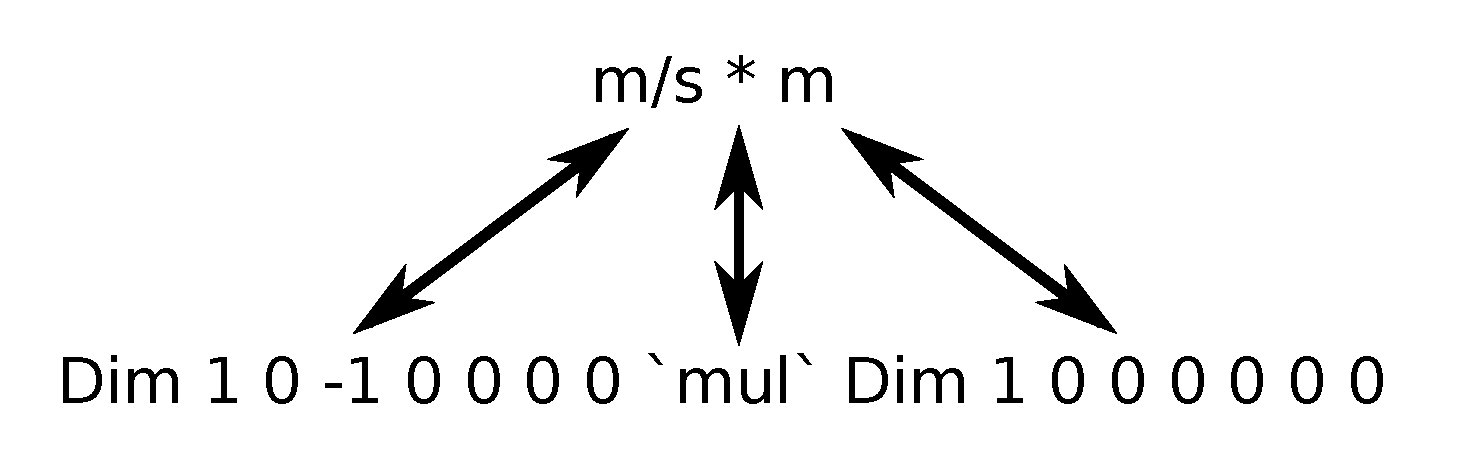
\includegraphics[width=0.6\linewidth]{figure/haskell_fysik_likhet.pdf}}
  \caption{Jämförelse mellan fysikaliska dimensioner (övre raden) och
  motsvarande implementation i Haskell (undre raden). Implementationen kommer
från det resulterande läromaterialet. Mer om implementationen finns att läsa i
avsnitt~\ref{sec:grund_impl}}\label{fig:haskell_fysik_likhet}
\end{figure}

Anledningen till att vi tycker att dessa drag gör ett område mer eller
mindre lämpat för ett domänspecifikt språk kommer från det val vi gjorde tidigt
i projektet, nämligen valet att använda Haskell. I avsnitt~\ref{sec:syntax}
beskriver vi begreppen syntax, semantik och syntaxträd och dess koppling till
både domänspecifika språk och Haskell. Dock finns det ingenting som säger att
man måste lägga ett sådant stort fokus som vi har gjort på till exempel syntaxträd. Hade
vi istället valt bort Haskell till fördel för ett objektorienterat språk hade vår definition av vad som gör ett område lämpat för
implementation kanske sett helt annorlunda ut.

I kontrast till dessa lämpliga områden står mindre lämpliga områden (eller
åtminstone områden som vi inte lyckades göra något bra av). Lutande plan är ett exempel på ett mindre lämpligt område. Områden av detta slag har drag som gör det mindre lämpligt än exempelvis vektorer.

När man skapar ett domänspecifikt språk till ett område gör man det genom att
identifiera syntaxen som används, datan som modelleras,
vilka operationer som används på denna data och vad det finns för lagar och samband
som gäller för dessa. Detta sätt att arbeta fungerar bra för områden som är
generella och som går att modellera på ett sätt som tillåter vidareutveckling, såsom
vektorer i flera dimensioner eller vektorer vars komponenter kan vara av vilken
typ som helst.

Ett exempel på ett område som inte har några tydliga data och operationer är
lutande plan. Ett sådant område har istället teoretiska samband som relaterar
olika egenskaper i systemet till varandra. Ett sådant samband är till exempel $a
= g \cdot \sin(v)$ för det lutande planet i figur~\ref{fig:lutande_plan}.

\begin{figure}[tph]
  \centering
  \frame{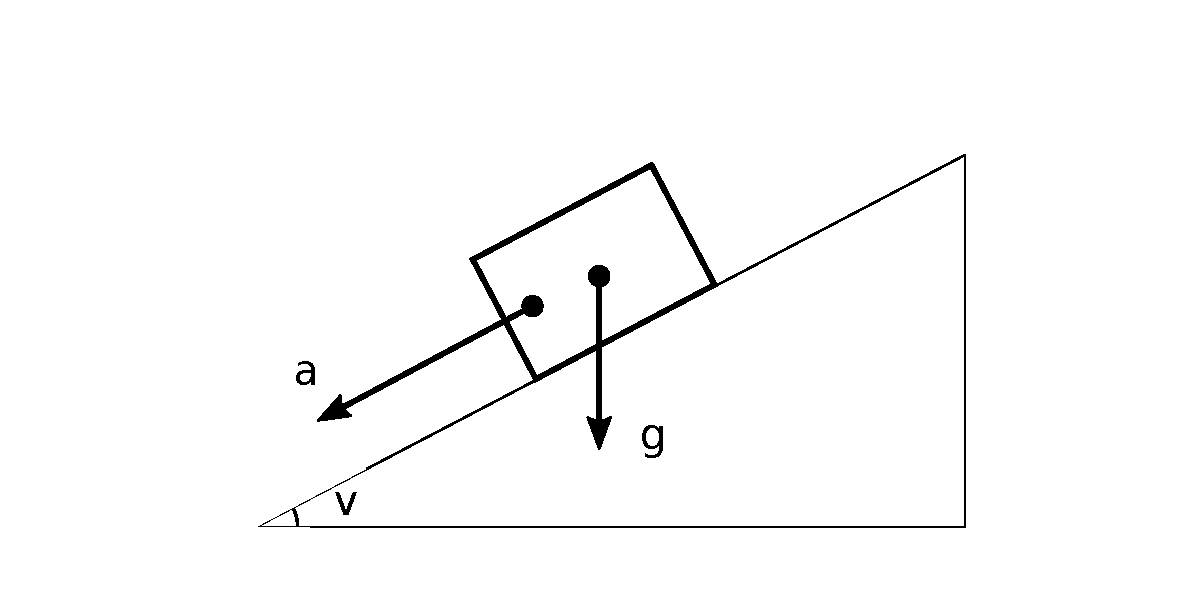
\includegraphics[width=0.5\linewidth]{figure/Lutande_plan.pdf}}
  \caption{Den variant av lutande plan som refereras till i exemplet i texten. $a$
  är en lådas acceleration längs med planet, $g$ är tyngdacceleration och $v$ är
  vinkeln. Friktionen antas vara försumbar.}~\label{fig:lutande_plan}
\end{figure}

Samband och ekvationer av detta slag kan visserligen modelleras som ett domänspecifikt
språk, men vi menar att nyttan inte blir stor med det eftersom allt vi då gör är
att skriva de formler som redan finns att tillgå i diverse kursböcker i fysik
utan att tillföra någon ny kunskap och utan att modellera dem på ett generellt
eller unikt sätt. Det man då kan göra är att programmera en ekvationslösare men
den hade varit både mekanisk och komplex. Den skulle alltså skilja sig
drastiskt från hur man löser problem för hand och skulle vara svår att förstå.
Alldeles för mycket fokus skulle hamna på algoritmer istället för fysik. Vi
anser även att en ekvationslösare inte hjälper till att lära ut fysik, tvärtom
döljer den matematiken som ligger bakom svaret.

När det kommer till lutande plan och liknande områden är nyckeln att visserligen
känna till vilka samband som gäller, men det är framförallt att veta när man ska
använda dem och hur man tillämpar dem på olika typer av uppgifter. Vi behandlar
därför områden som lutande plan genom att lösa exempeluppgifter modellerade i de
tidigare domänspecifika språk. De tidigare språken tillhandahåller de matematiska
verktyg som behövs för att koda upp lösningar av problem. Därav innehåller det
resulterande läromaterialet, som beskrivs i avsnitt~\ref{sec:res_laromaterial},
inga domänspecifika språk för fysikaliska problem.

Att vissa områden var mindre lämpliga var ett oväntat resultat i projektets
genomförande. Vid start trodde vi att det skulle gå att göra domänspecifika
språk för alla områden, såväl matematiska som fysikaliska, men som vi
diskuterat här gick inte det. Istället gjordes uppdelningen mellan grundläggande och
komposita områden, som beskrevs i avsnitt~\ref{sec:valet}, så att de fysikaliska
områden (som blev komposita) kunde behandlas som tillämpningar av de
grundläggande områdena.

\subsection{Domänspecifika språk, fysik och pedagogiska aspekter}\label{sec:bara_fysik}

En del av projektets mål är att diskutera huruvida det finns en pedagogisk nytta i att kombinera fysik och domänspecifika språk. Denna fråga diskuteras nedan.

Domänspecifika språk kan betraktas som ``tools for thinking''\footnote{Uttryckt i Patrik Janssons egna ord, han är föreläsare i DSLsofMath-kursen.}. Med det menas att domänspecifika språk kan användas
till att strukturera ett område så att det blir enklare att få en överblick och
förstå det. Dimensioner i läromaterialet är ett bra exempel på
detta, se även avsnitt~\ref{sec:grund_impl}. Där konstateras att en godtycklig
dimension kan skrivas som de sju grunddimensionerna med tillhörande exponenter.
Eftersom dimensionerna måste definieras så tydligt att det går att göra ett
program av det tvingas man att ge struktur till dem. Det ger ett nytt,
välstrukturerat och förhoppningsvis enklare sätt att se på dem, vilket vi själva
tycker är meningsfullt.

År 2016 genomfördes ett kandidatarbete på Chalmers liknande
detta~\cite{kandidat2016}. Det kandidatarbetet resulterade också i ett
läromaterial. Skillnaden är att det handlade om signallära medan detta handlar
om fysik. Grundidén är dock densamma: att använda domänspecifika språk för att
ge struktur till ett annat område.  Detta tycker vi visar på att det finns ett
akademiskt intresse för att använda domänspecifika språk i syfte att lära ut,
och att det inte bara är fysik och matematik som är lämpliga områden utan att
den generella idén som vi presenterar i denna rapport även går att applicera på
andra områden. Nyttan med att strukturera upp områden i väl avgränsade och
tydligt definierade delar kanske anses som uppenbar, men frågan om med vilket
verktyg man ska utföra detta är inte lika uppenbar. Vi hävdar att domänspecifika
språk är ett sådant verktyg och att det även är ett mycket bra verktyg att
använda sig av.

En annan aspekt är att när de domänspecifika språken används till fysikalisk
problemlösning måste det ske enligt de regler som ställdes upp när de
domänspecifika språken definierades. Det går med andra ord inte att fuska och ta
genvägar i beräkningarna. Detta tankesätt tycker Fäldt, se
avsnitt~\ref{sec:res_ake}, är en mycket bra aspekt som förmedlas med att
presentera fysik på detta sätt. Studenten skolas in i att tänka i rigorösa och
kompletta banor.

Det som talar emot
domänspecifika språk när det kommer till fysik är den stora del av problemlösning
som ingår i fysik. Det har att göra med deras olika natur. Domänspecifika språk
har en entydig och fyrkantig struktur medan problemlösning handlar om
kreativitet och nytänkande för att bygga upp modeller. Eftersom en stor del i fysik är just problemlösning
kan denna del inte fångas upp med domänspecifika språk. Det skulle till och med
kunna vara en nackdel att kombinera domänspecifika språk och fysik om det leder
till att man tänker alltför fyrkantigt kring fysik. Vi anser dock att
domänspecifika språk har ett värde ihop med fysik just för dessa strukturgivande
möjligheter, även om inte alla aspekter av fysik kan täckas.

Man kan också
tänka sig att det finns ett värde i omsluta den kreativa problemlösningen
med ett fyrkantigt system och på så sätt stoppa problemlösaren från att göra
misstag. På ett förenklat sätt kan man säga att så länge typsystemet inte klagar
betyder det att man löser problemet på ett korrekt sätt. Igen handlar det om att se
domänspecifika språk som ``tools for thinking'' och inte att vårt
läromaterial kommer att ge alla svaren när det kommer till fysikalisk
problemlösning. Men vad det kan tillföra är en struktur som kan hjälpa
läsaren att enklare komma fram till lösningen, och som garanterar att inga
syntaktiska misstag gjorts.

Hittills har domänspecifika språk framförts som ett sätt att strukturera fysik.
Projektets läromaterial är ett exempel på ett sådant försök. Men läromaterialet
har även haft två andra drag förutom domänspecifika språk, som skiljer sig från
traditionell fysikundervisning, nämligen ett lättillgängligt språk och en
nogrann genomgång av koncepten. Genom att enbart ha fokus på fysik är det möjligt att fysiken i sig hade kunnat förklarats bättre än vad den gör nu. Ett
läromaterial om renodlad fysik med ett lättsamt språk och nogrann förklaring av
koncepten hade säkert varit uppskattat. Khan Academy är ett sådant
exempel~\cite{khan} och som är mycket uppskattat. En annan fördel hade varit att en större målgrupp kan nås.
Men då missar man de saker domänspecifika språk bidrar med, nämligen det som
diskuterats ovan: att ge struktur och att lära ut ett rigoröst tankesätt. Man
missar också den \textit{intresseväckande} potentialen.

Domänspecifika språk kan ses som ett sätt göra fysik intressantare. Tycker man
att domänspecifika språk är roligt men inte fysik skulle en överbryggning av dem
kunna leda till att man tycker fysik blir roligare. Detta genom att man ser
parallellerna mellan domänspecifika språk och fysik. Ett exempel är typsystemet i
Haskell och dimensioner i fysik. I bägge världarna får inte olika typer
respektive dimensioner adderas, och vid operationer behandlas de på liknande
sätt. Denna likhet påvisades i läromaterialet genom att implementera fysikaliska
dimensioner i Haskells typsystem, se avsnitt~\ref{sec:res_laromaterial}. Denna
tanke stöds även av att testgruppen tyckte läromaterialet var ett intressant sätt
att presentera fysik på och att vi var inne på rätt spår i vår utformning av
läromaterialet, se avsnitt~\ref{sec:res_test}. Eftersom utvärderingen med
testgruppen var väldigt kort är det dock svårt att dra några säkra slutsatser
med hjälp av den. Nyttan med ett större intresse för fysik är att man
då förhoppningsvis är mer motiverad att klara fysikkurserna.

Avslutningsvis när det kommer till de domänspecifika språkens varande eller
icke-varande
ihop med fysikundervisning anser vi att en antingen-eller syn inte är konstruktiv.
Istället kan man kombinera dem på ett mer balanserat sätt. Det kan handla om att ha
vissa inslag av domänspecifika språk i en annars traditionell fysikundervisning,
och på så sätt fånga upp de delar domänspecifika språk gör bra i fysik:
strukturera, uppmuntra rigorös problemlösning och väcka intresse. Men samtidigt
förlita sig på traditionella metoder till stor del i bland annat problemlösning
och inte låta fokuset glida för långt från fysik till domänspecifika språk.

\section{Vidareutvecklingsmöjligheter och behov av ytterligare kunskap}

Läromaterialet innehåller domänspecifika språk för de \textit{matematiska}
områdena analys och vektorer. Dessa områden används sedan för att koda upp och
lösa uppgifter av mer \textit{fysikaliska} slag, till exempel krafter på lådor. Med andra ord hanteras fysikaliska områden genom att \textit{tillämpa} matematiska domänspecifika språk och inte genom att \textit{konstruera} fysikaliska domänspecifika språk. En vidareutveckling
hade därmed varit att göra precis det, att inte tillämpa matematiska
domänspecifika språk utan att göra fysikaliska domänspecifika språk. Det kan till exempel vara
saker som ett språk för ett lutande plans komponenter, ett språk för vilka krafter som verkar på fysikaliska kroppar i mekanikproblem eller till och med ett språk för något så abstrakt som
fysikalisk problemlösning i allmänhet. Vi vet inte hur ett domänspecifikt språk
av detta slag kan se ut, vilket är anledningen till att vi gick den andra vägen,
som vi diskuterade i avsnitt~\ref{sec:fpf}. Att göra fler fysikorienterade
domänspecifika språk hade därför varit en möjlig vidareutveckling.

En annan möjlig vidareutveckling är att göra en rigorös studie kring de
pedagogiska aspekterna hos kombinationen av fysik och domänspecifika språk.
Detta projekt innehöll enbart en mindre sådan studie. Det som kan vara
intressant att undersöka är om studenter tycker att fysik blir intressantare
genom en kombination av detta slag och kanske därför studerar mer i fysikkursen.
Det hade också varit intressant att undersöka om det rigorösa tankesätt
domänspecifika språk förmedlar (se avsnitt~\ref{sec:bara_fysik}) spiller över och
gör nytta inom traditionell fysikundervisning. Det är för dessa två frågor det
främsta behovet av ytterligare kunskaper ligger. Ett av målen med detta projekt var trots allt att förbättra fysikkunskaper (genom ökat intresse eller mer
rigorösitet) och då är det viktigt att undersöka om det faktiskt blir
så i praktiken.

Även det befintliga läromaterialet kan byggas vidare på. I sin nuvarande
form behandlas varken termodynamik eller vågrörelselära alls. Dessutom
finns det aspekter inom den klassiska mekaniken som fattas.

Slutligen finns det en mycket intressant vidareutveckling som inte alls har
behandlats i detta projekt, nämligen att använda matematiska och fysikaliska domänspecifika språk som
ett syntaktiskt lager mellan användare och en underliggande komplex kodbas. I
många fall kan dessa kodbaser vara implementerade på sätt som inte förefaller vara intuitivt, och saknar
typsäkerhet. I dessa fall kan det vara användbart med ett
domänspecifikt språk med hög typsäkerhet som tvingar användaren att
endast skriva korrekta uttryck och som döljer den bakomliggande komplexiteten. Tänk till exempel på kod i Matlab. Där är det lätt hänt att missa någon detalj i sin implementation så att beräkningarna blir fel utan att Matlab klagar. Uttrycket är korrekt men semantiken är fel. Med ett syntaktiskt lager som kräver att de fysikaliska dimensionerna stämmer överens hade vissa misstag kunnat upptäckas vid kompilering istället för att kanske inte upptäckas alls. Denna idé framfördes till oss av Jeff Chen\footnote{Jeffs sida på Chalmers:
\url{http://www.cse.chalmers.se/\~yutingc/}.}
på Chalmers, men är även någonting som har genomförts på andra områden, till
exempel inom molekylär dynamik~\cite{MD}.

\section{Etiska aspekter}

En bakomliggande tanke vi haft genom hela projektet är att läromaterialet ska
vara fritt tillgängligt för alla, därför har vi valt att publicera det på en
hemsida.  Denna hemsida använder grundläggande HTML och CSS samt javascript.
Javascript är dock inget strikt krav för funktionaliteten. Eftersom hemsidan är
lättviktig bör den fungera väl även på gamla datorer och telefoner, till
skillnad från tunga PDF-filer och många moderna hemsidor. Läromaterialet blir på
detta sätt tillgängligt även för studenter i länder med sämre
internetuppkoppling.

Tanken om tillgänglighet ligger även bakom valet att låta källkoden vara fritt
tillgänglig. Visserligen \textit{är} läromaterialet i princip hela källkoden, det vill säga
har man läromaterialet har man källkoden. Men att ha tillgång till källkoden
direkt har dock fördelar som att man kan följa med i versionshistoriken, man kan
se kommentarer och alternativa implementationer som inte syns i den slutgiltiga
produkten samt att det blir enklare att modifiera källkoden och lära sig om
hemsidans uppbyggnad.  Det handlar om transparens, att visa att man är positiv till att andra
tittar på hur man gjort och låta dem bygga vidare på ens skapelser. Genom att
sluta oss till skaran som skapar öppen källkod hoppas vi att fler inom samhället
i stort ska gå över till denna modell.

Valet att skriva på engelska har också att göra med tillgängligheten. Fler kan
engelska än svenska. På detta sätt kan läromaterialet komma fler till gagn.

Angående ambitionerna att upplevelsen av materialet är ämnad att
vara rolig, så är det mer tillgängligt för elever som kanske inte hade orkat
läsa en akademisk lärobok. Även om kvalitén i en akademisk lärobok kan vara hög,
är det inte alltid kvalitén kommer till nytta om eleven lägger boken åt sidan på
grund av en impuls att göra något som kan vara mer stimulerande.  Genom att
använda ett enkelt språk, roliga formuleringar och bilder, minskar chansen för
flyktförsök. Detta kan tänkas vara extra viktigt för yngre elever vars kontroll
av uppmärksamhet inte är lika utvecklad som hos äldre, men som ändå är
intresserade av fysik på en mer avancerad nivå än de studerar i sin ordinarie
undervisning.



\chapter{Slutsatser}

Projektets mål var att konstruera ett läromaterial som modellerar fysik med
hjälp av domänspecifika språk samt att diskutera hur väl det fungerar och om det finns en
pedagogisk nytta i det. Bakgrunden låg i att projektgruppen ville väcka intresse
för fysik hos datastudenter genom att presentera det ur ett 
programmeringsperspektiv. Det skulle förhoppningsvis kunna förbättra den mindre
bra tentastatistiken i kursen Fysik för ingenjörer.

Resultatet blev ett läromaterial bestående av domänspecifika språk i Haskell
sammanvävt med en lärotext som förklarar dem. Det innehåller kapitel för
dimensioner, matematisk analys, partikelmekanik, vektorer och tillämpningar av
dem på fysikaliska problem. Det ingår även programmeringsövningar.
Läromaterialet publicerades på en hemsida som är fritt tillgänglig för alla att
besöka.

För att undersöka den pedagogiska nyttan hölls två möten med Åke Fäldt, föreläsare och examinator för Fysik
för ingenjörer. Det framgick från mötena med Fäldt att det fanns en klar
pedagogisk nytta med det tillvägagångssätt som vi använt för att beskriva fysik.
Den rigorösa struktur som Haskell tvingar en att använda ger inte utrymme för en
student att hoppa över delar av förståelsen för ett fysikproblem. Istället
tvingas studenten att implementera hela lösningen från grunden och detta kan
ge en djupare förståelse för problemet och fysiken i stort. 

Det faktiska resultatet från detta tillvägagångssätt, läromaterialet,
testades av en testgrupp. Från denna grupp fick vi mycket positiv kritik och de
tyckte att läromaterialet var pedagogiskt, roligt och intressant. Men för att
verkligen kunna dra några slutsatser från detta krävs en mycket mer nogrann
undersökning huruvida studenter blir bättre på fysik med hjälp av ett
läromaterial av detta slag.

Till sist vill vi säga vi anser att det material vi har producerat har följt våra mål väl eftersom det är roligt, lättläst och intressant. Och även om den pedagogiska nyttan av materialet inte är ordentligt testat tycker vi alla i projektgruppen att vi har dragit stor nytta av att utveckla det.



% REFERENCES / BIBLIOGRAPHY
\cleardoublepage
\addcontentsline{toc}{chapter}{Bibliography}
\bibliographystyle{ieeetran}
\bibliography{include/backmatter/referenser}

% APPENDICES
\cleardoublepage
\appendix
\setcounter{page}{1}
\pagenumbering{Roman} % Capitalized roman numbering starting from I (one)

\chapter{Bilaga $\lambda$}

\section*{Inläsning}

\begin{itemize}
    \item Identifikation av problemområden.
        \begin{itemize}
            \item Kontakt med Åke Fäldt och DNS. Studera kursutvärderingar.
            \item Reflektera över vad vi själva tyckt varit svåra områden då vi
          läst kursen.  \end{itemize}
    \item Studerande av existerande läromaterial, både inom ren fysik och liknande vårt material.
        \begin{itemize}
            \item Fysikboken.
            \item Åke Fäldts egna material.
            \item Boken \textit{Structure Interpretaton of Classical Mechanics}\cite{SICM}.
            \item Kursboken till kursen \textit{Matematikens domänspecifika språk}.
        \end{itemize}
    \item Existerande implementationer.
        \begin{itemize}
            \item OpenTA.
            \item Hamilton.
            \item MasteringPhysics.
        \end{itemize}
    \item Tidigare forskning.
        \begin{itemize}
            \item Cezar och Patriks 2015 forskningsartikel.
            \item 2016 års kandidatarbete.
            \item Artikeln \textit{DSL for the Uninitiated}.
            \item \textit{Communicating Mathematics: Useful Ideas from Computer Science}
        \end{itemize}
\end{itemize}

\section*{Implementation av domänspecifika språk}

Vid implementationen av ett/flera domänspecika språk behöver nedanstående punkter genomföras.

\begin{itemize}
    \item Hitta relevanta grundtyper inom fysik, exempelvis sträcka och massa.
    \item Hitta relevanta komposittyper, exempelvis hastighet och tryck.
    \item Utförligt typsystem.
    \item Dimensionskontroll.
    \item Modellera fysikens syntax i språket.
    \item Pedagogiska syntaxträd.
    \item Kombinatorer och konstruktorer.
    \item Hålla våra typer polymorfa.
\end{itemize}

\section*{Skrivande av läromaterial}

Vid skrivandet av läromaterialet kommer följande punkter ligga till grund.

\begin{itemize}
    \item En gemensam vokabulär som fungerar när man skriver om både
      fysik och programmering (generics kontra polymorfism), och som gör det
      möjligt att prata om dem i samma mening utan att byta språk och på så sätt
      brygga det semantiska gapet mellan områdena.  
    \item Övningar
        \begin{itemize}
            \item Modellera ett fysikaliskt problem med vårt domänspecifika språk.
            \item Lös ett ''vanligt'' fysikaliskt problem med hjälp av vårt domänspecifika språk.
            \item Simuleringar i stil med \textit{Bouncing Balls}.
            \item Delar av fysiken vi inte behandlat lämnas som övning att själv implementera.
        \end{itemize}
    \item Gå igenom allmän teori (t.ex. Newtons lagar, krafter som verkar, etc) tillsammans med en parallell utveckling av ett domänspecifikt språk.
    \item Materialet ska vara enkelt att ta till sig.
    \item Verkligen exponera det DSL som vi gemensamt bygger för att påvisa kopplingen mellan fysik och programmering.
\end{itemize}



\end{document}
